% ============================================================
%  chapter01.tex — 第一章 基本定理
%  对应原书第一章。
%  本章建立全书的基础：解的存在唯一性、延拓、动力系统概念、
%  以及平面动力系统。
% ============================================================

\setchapterimage{}
\setchapterintro{}
\chapter{基本定理}
\renewcommand{\thesection}{\arabic{section}}
\newcommand{\sourceSection}[1]{%
  \refstepcounter{section}%
  \section*{\S\ \arabic{section}.\ #1}%
  \addcontentsline{toc}{section}{\arabic{section}. #1}%
}

本章介绍关于微分方程的解的一些基本定理，这是常微分方程一般理论的基础。

% ============================================================
%  §1  解的存在性、唯一性及对初值(或参数)的依赖性
% ============================================================
\sourceSection{解的存在性、唯一性及对初值(或参数)的依赖性}

\begin{theorem}{}{cauchy-exist}
	考虑 Cauchy 问题 $(E)$：
	\[
		\begin{cases}
			\dfrac{\dd \vect{x}}{\dd t} = \vect{f}(t,\vect{x}), \\[4pt]
			\vect{x}(t_0) = \vect{x}_0,
		\end{cases}
		\tag{1.1}
	\]
	其中 $\vect{x}$ 是 $\R^n$ 中的向量，$\vect{f}(t,\vect{x})$ 是实变量 $t$ 和 $n$ 维向量 $\vect{x}$ 的 $n$ 维向量值函数；又设 $\vect{f}(t,\vect{x})$ 在闭区域 $G$：
	\[
		|t - t_0| \leq a, \qquad \|\vect{x} - \vect{x}_0\| \leq b,
	\]
	上连续，并且对 $\vect{x}$ 适合 Lipschitz 条件：
	\[
		\|\vect{f}(t,\vect{x}_1) - \vect{f}(t,\vect{x}_2)\| 
		\leq L\|\vect{x}_1 - \vect{x}_2\|,
		\quad (t,\vect{x}_i) \in G,\ i = 1,2,
		\tag{1.2}
	\]
	其中 Lipschitz 常数 $L>0$。令
	\[
		M = \max_G \|\vect{f}(t,\vect{x})\|, \qquad 
		h = \min\!\left(a,\ \frac{b}{M}\right).
		\tag{1.3}
	\]
	那末 Cauchy 问题 $(E)$ 在区间 $|t-t_0|\leq h$ 上有一个解 $\vect{x}=\vect{\varphi}(t)$，并且它是唯一的。
\end{theorem}

\begin{proof}
	我们分以下五个步骤证明之。

	\textbf{（一）Cauchy 问题 $(E)$ 等价于积分方程}
	\[
		\vect{x} = \vect{x}_0 + \int_{t_0}^t \vect{f}(t,\vect{x})\,\dd t.
		\tag{1.4}
	\]

	事实上，令 $\vect{x} = \vect{\varphi}(t)$ 是 Cauchy 问题 $(E)$ 的解，于是由 (1.1) 对 $t$ 积分便有
	\[
		\vect{\varphi}(t) = \vect{C} + \int_{t_0}^t \vect{f}(t,\vect{\varphi}(t))\,\dd t,
	\]
	再由初值条件 (1.2) 确定 $\vect{C} = \vect{x}_0$，因此 $\vect{x} = \vect{\varphi}(t)$ 是（E）的解。

	反之，设 $\vect{x} = \vect{\varphi}(t)$ 是积分方程 (1.4) 的解，从 (1.4) 可知 $\vect{\varphi}(t)$ 是连续的，从而 $\vect{f}(t,\vect{\varphi}(t))$ 也是连续的，因此 $\vect{\varphi}(t)$ 是可微的；于是，对积分方程 (1.4) 的两侧对 $t$ 求导数，便得到
	\[
		\vect{\varphi}'(t) = \vect{f}(t,\vect{\varphi}(t)),
	\]
	并且由 (1.4) 可见 $\vect{x} = \vect{\varphi}(t)$ 满足初值条件
	\[
		\vect{\varphi}(t_0) = \vect{x}_0,
	\]
	即 $\vect{\varphi}(t)$ 是 Cauchy 问题 $(E)$ 的解。

	\textbf{（二）作 (1.4) 的 Picard 近似解序列 $\{\vect{\varphi}_n(t)\}$}

	令 $\vect{\varphi}_0(t) \equiv \vect{x}_0$，
	\[
		\vect{\varphi}_1(t) = \vect{x}_0 + \int_{t_0}^t \vect{f}(t,\vect{x}_0)\,\dd t,\quad
		|t - t_0| \leq h.
		\tag{1.5}
	\]
	则
	\[
		\|\vect{\varphi}_1(t) - \vect{\varphi}_0(t)\| 
		\leq \left|\int_{t_0}^t \|\vect{f}(t,\vect{x}_0)\|\,\dd t\right|
		\leq M \cdot |t - t_0| \leq b.
		\tag{1.6}
	\]

	当 $\vect{x}$ 是一维时，图形如下：


\begin{center}
	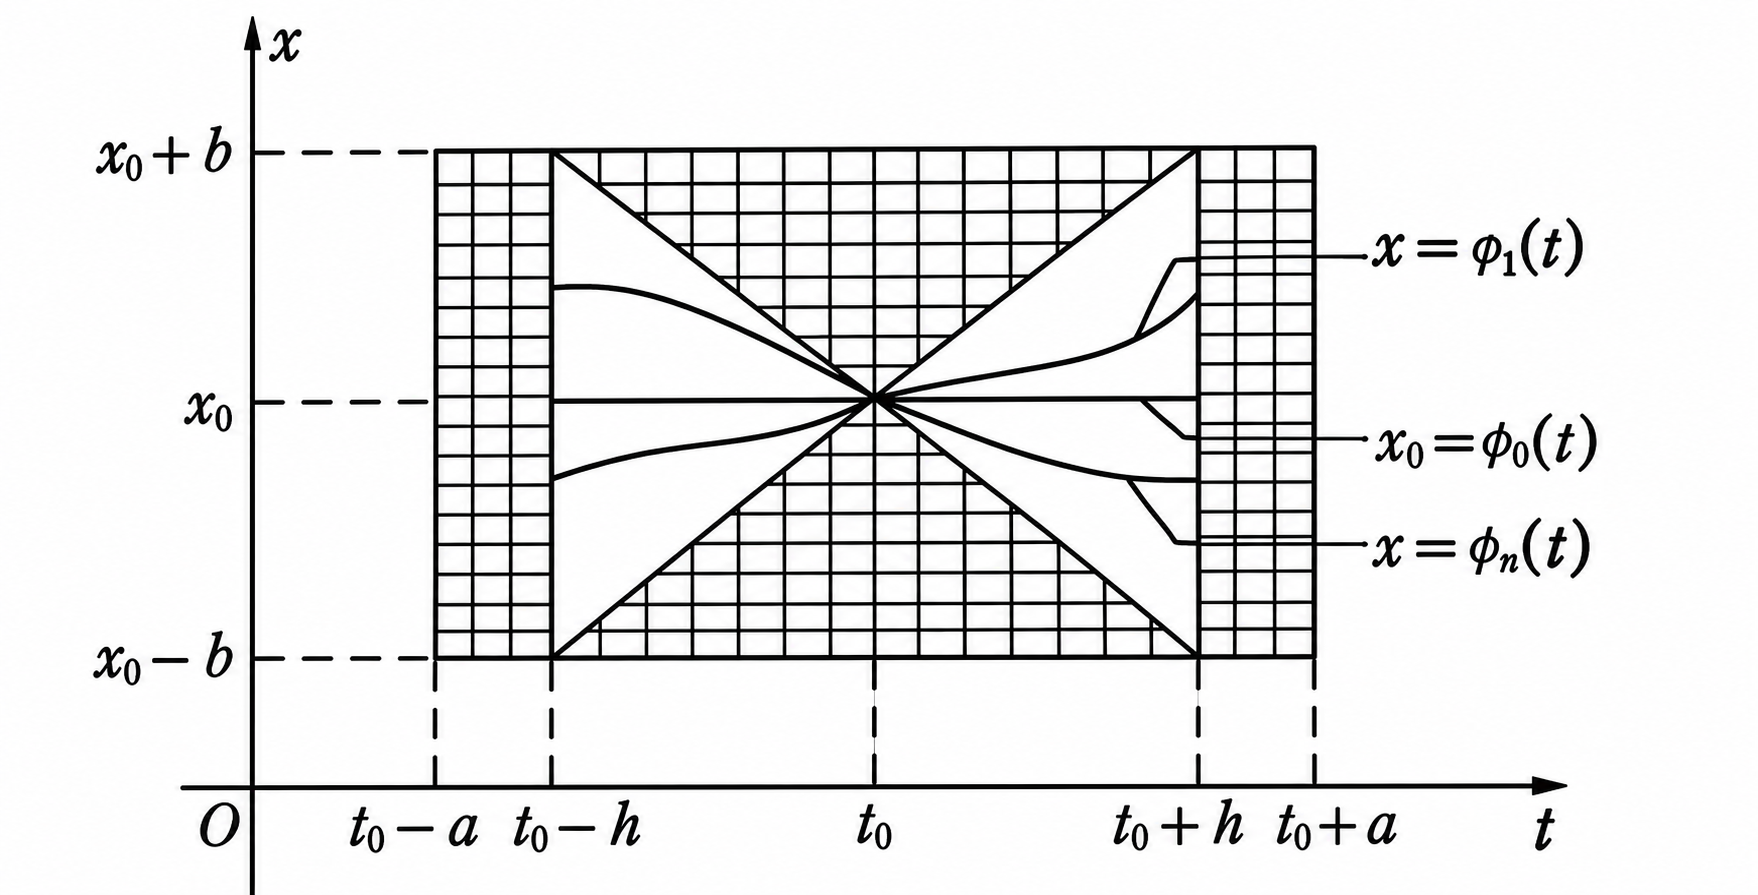
\includegraphics[width=0.7\linewidth]{figure/1}
	\captionof{figure}{}
\end{center}

	我们可以采用归纳的程序：设已得第 $n$ 次近似解为
	\[
		\vect{\varphi}_n(t) = \vect{x}_0 + \int_{t_0}^t \vect{f}(t,\vect{\varphi}_{n-1}(t))\,\dd t,
		\tag{1.7}
	\]
	而且当 $|t - t_0| \leq h$ 时，我们有
	\[
		\|\vect{\varphi}_n(t) - \vect{x}_0\| \leq b.
	\]
	令第 $n + 1$ 次近似解为
	\[
		\vect{\varphi}_{n+1}(t) = \vect{x}_0 + \int_{t_0}^t \vect{f}(t,\vect{\varphi}_n(t))\,\dd t,
		\tag{1.8}
	\]
	则当 $|t - t_0| \leq h$ 时，我们有
	\begin{align*}
		\|\vect{\varphi}_{n+1}(t) - \vect{x}_0\|
		&\leq \left\|\int_{t_0}^t \vect{f}(t,\vect{\varphi}_n(t))\,\dd t\right\| \\
		&\leq M \cdot |t - t_0| \leq Mh \leq b, \quad n = 1, 2, 3,\cdots.
	\end{align*}

	\textbf{（三）序列 $\{\vect{\varphi}_n(t)\}$ 的一致收敛性}

	由于 $\{\vect{\varphi}_n(t)\}$ 的收敛问题等价于级数
	\begin{align*}
		&\vect{\varphi}_0(t) + [\vect{\varphi}_1(t) - \vect{\varphi}_0(t)] 
		+ [\vect{\varphi}_2(t) - \vect{\varphi}_1(t)] \\
		&+ \cdots + [\vect{\varphi}_n(t) - \vect{\varphi}_{n-1}(t)] + \cdots
		\tag{1.9}
	\end{align*}
	的收敛问题，我们只要证明 (1.9) 的一致收敛性即可。

	首先证明 (1.9) 的一般项满足
	\[
		\|\vect{\varphi}_n(t) - \vect{\varphi}_{n-1}(t)\| 
		\leq \frac{M}{L}\,\frac{(L|t - t_0|)^n}{n!}, \quad n = 1, 2, 3,\cdots.
		\tag{1.10}
	\]
	由 (1.6) 可知 (1.10) 对 $n = 1$ 成立。假设不等式 (1.10) 对 $n = m$ 成立，则我们有下述不等式：
	\begin{align*}
		\|\vect{\varphi}_{m+1}(t) - \vect{\varphi}_m(t)\|
		&= \left\|\int_{t_0}^t \bigl(\vect{f}(t,\vect{\varphi}_m(t)) 
			- \vect{f}(t,\vect{\varphi}_{m-1}(t))\bigr)\,\dd t\right\| \\
		&\leq L \cdot \left|\int_{t_0}^t \|\vect{\varphi}_m(s) - \vect{\varphi}_{m-1}(s)\|\,\dd t\right| \\
		&\leq \frac{M}{L}\,\frac{(L|t - t_0|)^{m+1}}{(m+1)!}.
	\end{align*}
	由此可知不等式 (1.10) 对所有正整数 $n$ 都成立。所以当 $|t - t_0| \leq h$ 时，我们得到
	\[
		\|\vect{\varphi}_n(t) - \vect{\varphi}_{n-1}(t)\| 
		\leq \frac{M}{L}\,\frac{(Lh)^n}{n!}.
		\tag{1.11}
	\]
	由 Weierstrass 判别法推出级数 (1.9) 是一致收敛的，从而序列 $\{\vect{\varphi}_n(t)\}$ 一致收敛。令 $\lim_{n \to \infty} \vect{\varphi}_n(t) = \vect{\varphi}(t)$，则 $\vect{x} = \vect{\varphi}(t)$ 连续，且 $\|\vect{\varphi}(t) - \vect{x}_0\| \leq b\ (|t - t_0| \leq h)$。

	\textbf{（四）证明 $\vect{x} = \vect{\varphi}(t)$ 是积分方程 (1.4) 的解}

	令 $n \to +\infty$，由 (1.8) 得
	\[
		\vect{\varphi}(t) = \vect{x}_0 + \lim_{n \to \infty} \int_{t_0}^t 
			\vect{f}(t,\vect{\varphi}_n(t))\,\dd t.
		\tag{1.12}
	\]
	因此，归结于证明
	\[
		\lim_{n \to \infty} \int_{t_0}^t \vect{f}(t,\vect{\varphi}_n(t))\,\dd t 
		= \int_{t_0}^t \vect{f}(t,\vect{\varphi}(t))\,\dd t.
		\tag{1.13}
	\]
	任给 $\varepsilon > 0$，可找到 $N = N(\varepsilon) > 0$，使得当 $|t - t_0| \leq h$，便有不等式
	\[
		\|\vect{\varphi}_n(t) - \vect{\varphi}(t)\| \leq \frac{\varepsilon}{Lh}, 
		\quad \text{只要}\ n \geq N.
	\]
	因此，当 $|t - t_0| \leq h$ 时，我们有
	\begin{align*}
		&\left\|\int_{t_0}^t \vect{f}(t,\vect{\varphi}_n(t))\,\dd t 
			- \int_{t_0}^t \vect{f}(t,\vect{\varphi}(t))\,\dd t\right\| \\
		&\leq L \cdot \left|\int_{t_0}^t \|\vect{\varphi}_n(s) - \vect{\varphi}(s)\|\,\dd s\right| \\
		&\leq L \cdot \frac{\varepsilon}{L \cdot h} \cdot h = \varepsilon,
	\end{align*}
	即 (1.13) 成立。因此由 (1.12) 和 (1.3)，可见 $\vect{x} = \vect{\varphi}(t)$ 是积分方程 (1.4) 的一个解（$|t - t_0| \leq h$）。

	\textbf{（五）最后证明 (1.4) 的解的唯一性}

	事实上，设 $\vect{x} = \vect{\varphi}(t)$ 与 $\vect{x} = \vect{\psi}(t)$ 是 (1.4) 的两个解，即
	\[
		\vect{\varphi}(t) = \vect{x}_0 + \int_{t_0}^t \vect{f}(t,\vect{\varphi}(t))\,\dd s,
	\]
	与
	\[
		\vect{\psi}(t) = \vect{x}_0 + \int_{t_0}^t \vect{f}(t,\vect{\psi}(t))\,\dd t.
	\]
	两式相减，再利用 Lipschitz 条件，我们得到
	\[
		\|\vect{\varphi}(t) - \vect{\psi}(t)\| 
		\leq L \cdot \left|\int_{t_0}^t \|\vect{\varphi}(s) - \vect{\psi}(s)\|\,\dd t\right|.
		\tag{1.14}
	\]
	令
	\[
		g(t) = \int_{t_0}^t \|\vect{\varphi}(s) - \vect{\psi}(s)\|\,\dd t, \quad t \geq t_0.
	\]
	于是当 $t \geq t_0$ 时，$g(t) \geq 0$，而且 (1.14) 转化为
	\[
		g'(t) \leq L \cdot g(t),
		\tag{1.15}
	\]
	于是
	\[
		\bigl(e^{-L(t - t_0)} \cdot g(t)\bigr)' \leq 0,
	\]
	因而
	\[
		e^{-L(t - t_0)} \cdot g(t) \leq g(t_0) = 0.
	\]
	由此推出
	\[
		g(t) \equiv 0, \quad t \geq t_0,
	\]
	即
	\[
		\vect{\varphi}(t) \equiv \vect{\psi}(t), \quad t \geq t_0.
	\]
	同法可证：当 $t \leq t_0$ 时，$\vect{\varphi}(t) \equiv \vect{\psi}(t)$。

	总结以上各步骤，定理证毕。
\end{proof}

\fuzhu{1}{定理(1.1) 的证明是古典的，但可以抽象为泛函分析中的不动点定理。等式
\[
	\vect{\psi}(t) = \vect{x}_0 + \int_{t_0}^t \vect{f}(t,\vect{\varphi}(t))\,\dd t, 
	\quad |t - t_0| \leq h,
\]
定义了一个从连续函数 $\vect{\varphi}(t)$ 到连续函数 $\vect{\psi}(t)$ 的变换，可简写为
\[
	\vect{\psi} = \vect{T}(\vect{\varphi}).
\]
若 $\vect{T}(\vect{\varphi}) = \vect{\varphi}$，则称 $\vect{\varphi}$ 为变换 $\vect{T}$ 的不动点。显然 (1.4) 的解就是变换 $\vect{T}$ 的不动点。近代泛函分析中有各式各样的不动点定理，现介绍其中一个最简单的，称为\textbf{压缩映象原理}。

	设 $D$ 是 Banach 空间 $\mathscr{B}$ 的一个非空闭子集，$\vect{T}$ 是从 $D$ 到 $D$ 自身的映象，即对每一个 $\vect{\varphi} \in D$，有 $\vect{T}(\vect{\varphi}) \in D$。又存在常数 $k$，$0 \leq k < 1$，使对 $D$ 中任何两点 $\vect{\varphi}_1, \vect{\varphi}_2$，都有不等式
\[
	\|\vect{T}(\vect{\varphi}_1) - \vect{T}(\vect{\varphi}_2)\| \leq k\|\vect{\varphi}_1 - \vect{\varphi}_2\|.
\]
则在 $D$ 中存在唯一的一个点 $\vect{\varphi}^*$，使得 $\vect{T}(\vect{\varphi}^*) = \vect{\varphi}^*$。

	现在我们用上述压缩映象原理来证明定理(1.1)。取 $\mathscr{B}$ 为定义在区间 $|t - t_0| \leq a$ 上的一切连续函数所成的空间，取 $D$ 为定义在 $|t - t_0| \leq h^*$ 上 $\bigl(0 < h^* < \min(h, 1/L)\bigr)$ 而图象包含在 $G$ 中（见定理(1.1) 的条件）的一切连续函数所组成的集合。如果 $\vect{\varphi}(t) \in D$，定义
\[
	\vect{T}(\vect{\varphi}) = \vect{x}_0 + \int_{t_0}^t \vect{f}(\xi,\vect{\varphi}(\xi))\,\dd\xi,
\]
则
\[
	\|\vect{T}(\vect{\varphi}) - \vect{x}_0\| 
	\leq \left\|\int_{t_0}^t \vect{f}(\xi,\vect{\varphi}(\xi))\,\dd\xi\right\|
	\leq M|t - t_0| \leq Mh \leq b,
\]
即 $\vect{T}(\vect{\varphi}) \in D$。其次设 $\vect{\varphi}_1, \vect{\varphi}_2 \in D$，于是
\begin{align*}
	\|\vect{T}(\vect{\varphi}_1) - \vect{T}(\vect{\varphi}_2)\| 
	&\leq \left|\int_{t_0}^t \|\vect{f}(t,\vect{\varphi}_1) - \vect{f}(t,\vect{\varphi}_2)\|\,\dd t\right| \\
	&\leq L \cdot h^* \|\vect{\varphi}_1 - \vect{\varphi}_2\| \\
	&= K \|\vect{\varphi}_1 - \vect{\varphi}_2\|, \quad (K = Lh^* < 1).
\end{align*}
故由压缩映象原理，有唯一的不动点 $\vect{\varphi}^*$，使 $\vect{T}(\vect{\varphi}^*) = \vect{\varphi}^*$，即
\[
	\vect{\varphi}^*(t) = \vect{x}_0 + \int_{t_0}^t \vect{f}(t,\vect{\varphi}^*(t))\,\dd t, 
	\quad (|t - t_0| \leq h^*).
	\]
}

\fuzhu{2}{设方程 (1.1) 是线性的，即
\[
	\frac{\dd \vect{x}}{\dd t} = \vect{A}(t)\vect{x} + \vect{f}(t),
	\tag{1.16}
\]
其中 $\vect{A}(t), \vect{f}(t)$ 在区间 $[\alpha, \beta]$ 上是连续的。

这时由初值 $(t_0, \vect{x}_0)\ (t_0 \in [\alpha, \beta])$ 所确定的解在整个区间 $[\alpha, \beta]$ 上都有定义。这是因为所构造的逐次近似解序列 $\{\vect{\varphi}_n(t)\}$ 在整个区间 $[\alpha, \beta]$ 都有定义，并且是一致收敛的。}

\fuzhu{3}{如果 $\vect{f}(t, \vect{x})$ 对 $t, \vect{x}$ 连续，但不一定满足 Lipschitz 条件，则 Cauchy 问题 (1.1) + (1.2) 的解仍是存在的，参见下面的定理（证明从略）。}
\namedthm{Cauchy-Peano}{若 $\vect{f}(t, \vect{x})$ 在区域 $G: |t - t_0| \leq a, \|\vect{x} - \vect{x}_0\| \leq b$ 上连续，则 (1.4) 在区间 $|t - t_0| \leq h$ 上有解 $\vect{x} = \vect{\varphi}(t)$ 且满足初值条件 $\vect{\varphi}(t_0) = \vect{x}_0$，此处
	若 $\vect{f}(t, \vect{x})$ 在区域 $G: |t - t_0| \leq a, \|\vect{x} - \vect{x}_0\| \leq b$ 上连续，则 (1.4) 在区间 $|t - t_0| \leq h$ 上有解 $\vect{x} = \vect{\varphi}(t)$ 且满足初值条件 $\vect{\varphi}(t_0) = \vect{x}_0$，此处
\[
h = \min\!\left(a,\ \frac{b}{M}\right), \qquad 
M = \max_G \|\vect{f}(t,\vect{x})\|.
\]
}


下面讨论解与参数（或初值）的关系。

考虑方程
\[
	\begin{cases}
		\dfrac{\dd \vect{x}}{\dd t} = \vect{f}(t, \vect{x}), \\[4pt]
		\vect{x}(t_0) = \vect{x}_0,
	\end{cases}
\]
的解 $\vect{x} = \vect{\varphi}(t, t_0, \vect{x}_0)$。这个解是 $t, t_0, \vect{x}_0$ 的函数。例如方程
\[
	\begin{cases}
		\dfrac{\dd \vect{x}}{\dd t} = \vect{x}, \\[4pt]
		\vect{x}(t_0) = \vect{x}_0,
	\end{cases}
\]
的解为 $\vect{x} = \vect{x}_0 e^{t - t_0}$，它是 $t, t_0, \vect{x}_0$ 的函数。

这里发生了一个在理论上和应用上都很重要的问题：当初值或参数变动时，对应的解是如何变动的？我们知道，在应用上，微分方程是描述某种物理过程的。而将一个物理问题化成微分方程问题时，不论是初值还是参数，它们的数值都是由实验测定的，因此不可避免地会出现一些微小的误差。如果初值或参数的微小振动会引起方程的解发生剧烈的变化，那么所求解的可靠性就会很小。因此我们要研究 Cauchy 问题的解与初值或参数的关系是自然而必要的。

\begin{theorem}{}{param-cont}
	考虑 Cauchy 问题 $(E_{\vect{\mu}})$：
	\[
		\frac{\dd \vect{x}}{\dd t} = \vect{f}(t, \vect{x}, \vect{\mu}), \qquad 
		\vect{x}(t_0) = \vect{x}_0,
		\tag{1.17}
	\]
	此处 $\vect{x}$ 是 $\R^n$ 中的 $n$ 维向量，$\vect{\mu}$ 是 $\R^m$ 中的 $m$ 维向量。函数 $\vect{f}(t, \vect{x}, \vect{\mu})$ 在区域 $G$：
	\[
		|t - t_0| \leq a,\quad \|\vect{x} - \vect{x}_0\| \leq b,\quad \|\vect{\mu} - \vect{\mu}_0\| \leq c,
	\]
	上连续且对 $\vect{x}$ 适合 Lipschitz 条件：
	\[
		\|\vect{f}(t, \vect{x}_1, \vect{\mu}) - \vect{f}(t, \vect{x}_2, \vect{\mu})\| 
		\leq L\|\vect{x}_1 - \vect{x}_2\|, \quad \forall(t, \vect{x}_i, \vect{\mu}) \in G,\ i = 1,2,
	\]
	其中 Lipschitz 常数 $L > 0$。令
	\[
		M = \max_G \|\vect{f}(t, \vect{x}, \vect{\mu})\|, \qquad 
		h = \min\!\left(a,\ \frac{b}{M}\right),
	\]
	则对于任意 $\vect{\mu}\,(\|\vect{\mu} - \vect{\mu}_0\| \leq c)$，$(E_{\vect{\mu}})$ 的解 $\vect{x} = \vect{x}(t; \vect{\mu})$ 在区间 $|t - t_0| \leq h$ 上存在且唯一，并且 $\vect{x} = \vect{x}(t; \vect{\mu})$ 是 $(t, \vect{\mu})$ 的连续函数。
\end{theorem}

\begin{proof}
	对任意 $\vect{\mu}\,(\|\vect{\mu} - \vect{\mu}_0\| \leq c)$，根据定理~\ref{thm:cauchy-exist}，$(E_{\vect{\mu}})$ 的解 $\vect{x} = \vect{x}(t; \vect{\mu})$ 在 $|t - t_0| \leq h$ 上存在唯一。

	又因为 Cauchy 问题 $(E_{\vect{\mu}})$ 的 $n$ 次近似解 $\vect{x} = \vect{\varphi}_n(t; \vect{\mu})$ 是 $(t, \vect{\mu})$ 的连续函数而且当 $n \to +\infty$ 时，$\vect{\varphi}_n(t; \vect{\mu})$ 在区域 $(|t - t_0| \leq h, \|\vect{\mu} - \vect{\mu}_0\| \leq c)$ 上一致收敛，因而 $\vect{\varphi}(t; \vect{\mu})$ 是 $(t, \vect{\mu})$ 的连续函数。
\end{proof}

\namedlem{Grownwall}{设函数 $g(t), \varphi(t)$ 是区间 $[t_0, t_1]$ 上的连续函数，而且 $g(t) \geq 0, \varphi(t) \geq 0$；又常数 $\lambda > 0, r > 0$。若 $\varphi(t)$ 满足不等式
	设函数 $g(t), \varphi(t)$ 是区间 $[t_0, t_1]$ 上的连续函数，而且 $g(t) \geq 0, \varphi(t) \geq 0$；又常数 $\lambda > 0, r > 0$。若 $\varphi(t)$ 满足不等式
\[
\varphi(t) \leq \lambda + \int_{t_0}^t (g(t)\varphi(t) + r)\,\dd s, \quad t_0 \leq t \leq t_1,
\tag{1.18}
\]
则有
\[
\varphi(t) \leq (\lambda + rT)\,e^{\int_{t_0}^t g(s)\,\dd s}, \quad t_0 \leq t \leq t_1,
\tag{1.19}
\]
其中 $T = t_1 - t_0$。
}

\begin{proof}
	令 $u(t) = \varphi(t)\,e^{-\int_{t_0}^t g(s)\,\dd s}$，$t_0 \leq t \leq t_1$，显然 $u(t)$ 是连续的。设 $\xi = \sup\{u(t)\}_{t_0 \leq t \leq t_1}$，则存在 $t^* \in [t_0, t_1]$，使得 $u(t^*) = \xi$。由 (1.18) 得
	\begin{align*}
		\xi\,e^{\int_{t_0}^{t^*} g(s)\,\dd s} 
		&\leq \lambda + \int_{t_0}^{t^*} (g(s)\varphi(s) + r)\,\dd s \\
		&\leq \lambda + \int_{t_0}^{t^*} \bigl(\xi\,g(s)\,e^{\int_{t_0}^s g(s)\,\dd s} + r\bigr)\,\dd s \\
		&\leq \lambda + rT + \xi\bigl(e^{\int_{t_0}^{t^*} g(s)\,\dd s} - 1\bigr),
	\end{align*}
	即
	\[
		\xi \leq \lambda + rT.
	\]
	由于
	\[
		\varphi(t) \leq \xi\,e^{\int_{t_0}^t g(s)\,\dd s},
	\]
	故
	\[
		\varphi(t) \leq (\lambda + rT)\,e^{\int_{t_0}^t g(s)\,\dd s}.
	\]
\end{proof}

\begin{theorem}{}{param-diff}
	设 Cauchy 问题 $(E_{\vect{\mu}}^*)$：
	\[
		\frac{\dd \vect{x}}{\dd t} = \vect{f}(t, \vect{x}, \vect{\mu}), \qquad 
		\vect{x}(t_0) = \vect{x}_0,
	\]
	其中 $\vect{x}$ 是 $\R^n$ 中的 $n$ 维向量，$\vect{\mu}$ 是 $\R^m$ 中的 $m$ 维向量。又设 $\vect{f}(t, \vect{x}, \vect{\mu}) \in C^0(G, \R^n)$，其中
	\[
		G:\ |t - t_0| \leq a,\ \|\vect{x} - \vect{x}_0\| \leq b,\ \|\vect{\mu} - \vect{\mu}_0\| \leq c,
	\]
	且 $\dfrac{\partial \vect{f}}{\partial x_j}\ (j = 1, 2, \cdots, n)$，$\dfrac{\partial \vect{f}}{\partial \mu_k}\ (k = 1, 2, \cdots, m)$ 连续，则定理~\ref{thm:param-cont} 的结论成立，而且 $\vect{x} = \vect{x}(t, \vect{\mu})$ 对 $\mu_k\ (k = 1, 2, \cdots, m)$ 有连续的偏导数。
\end{theorem}

\begin{proof}
	因为 $\dfrac{\partial \vect{f}}{\partial x_j} \in C^0(G, \R^n)\ (j = 1, 2, \cdots, n)$，所以 $\vect{f}$ 对 $\vect{x}$ 适合 Lipschitz 条件。因此，定理~\ref{thm:param-cont} 蕴含定理~\ref{thm:param-diff}，即 $(E_{\vect{\mu}}^*)$ 的解 $\vect{x} = \vect{\varphi}(t, \vect{\mu})$ 存在唯一且在区域 $B(|t - t_0| \leq h, \|\vect{\mu} - \vect{\mu}_0\| \leq c)$ 上连续。下面证明 $\vect{x} = \vect{\varphi}(t, \vect{\mu})$ 对 $\vect{\mu}$ 是可微的。我们的证明分以下三个步骤进行。

	为了形式地推导 $\dfrac{\partial \vect{x}}{\partial \vect{\mu}}$，首先我们考虑线性方程
	\[
		\begin{cases}
			\dfrac{\dd \vect{z}}{\dd t} 
			= \vect{f}_{\vect{x}}(t, \vect{\varphi}(t, \vect{\mu}), \vect{\mu})\,\vect{z} 
			+ \vect{f}_{\vect{\mu}}(t, \vect{\varphi}(t, \vect{\mu}), \vect{\mu}), \\[4pt]
			\vect{z}(t_0) = \vect{0},
		\end{cases}
	\]
	或与上面等价的积分方程
	\[
		\vect{z}(t, \vect{\mu}) 
		= \int_{t_0}^t \bigl[\vect{f}_{\vect{x}}(t, \vect{\varphi}(t, \vect{\mu}), \vect{\mu})\,\vect{z}(t, \vect{\mu})
		+ \vect{f}_{\vect{\mu}}(t, \vect{\varphi}(t, \vect{\mu}), \vect{\mu})\bigr]\,\dd t,
		\tag{1.20}
	\]
	其中
	\[
		\vect{f}_{\vect{x}}(t, \vect{\varphi}(t, \vect{\mu}), \vect{\mu}) 
		= \left(\frac{\partial f_i(t, \vect{\varphi}(t, \vect{\mu}), \vect{\mu})}{\partial x_j}\right)_{n \times n}
	\]
	是 $n \times n$ 矩阵，
	\[
		\vect{f}_{\vect{\mu}}(t, \vect{\varphi}(t, \vect{\mu}), \vect{\mu}) 
		= \left(\frac{\partial f_i(t, \vect{\varphi}(t, \vect{\mu}), \vect{\mu})}{\partial \mu_k}\right)_{n \times m}
	\]
	是 $n \times m$ 矩阵。

	Cauchy 问题 $(E_0^{\vect{\mu}})$ 等价于积分方程
	\[
		\vect{x} = \vect{x}_0 + \int_{t_0}^t \vect{f}(t, \vect{x}, \vect{\mu})\,\dd t,
		\tag{1.21}
	\]
	从此式形式地计算 $\dfrac{\partial \vect{x}}{\partial \vect{\mu}}$ 得
	\[
		\frac{\partial \vect{x}}{\partial \vect{\mu}} 
		= \int_{t_0}^t \left(\frac{\partial \vect{f}(t, \vect{\varphi}(t, \vect{\mu}), \vect{\mu})}{\partial \vect{x}}\,\frac{\partial \vect{x}}{\partial \vect{\mu}}
		+ \frac{\partial \vect{f}(t, \vect{\varphi}(t, \vect{\mu}), \vect{\mu})}{\partial \vect{\mu}}\right)\dd t.
		\tag{1.22}
	\]
	这就是说，如果 $\dfrac{\partial \vect{x}}{\partial \vect{\mu}}$ 存在，则它应满足方程 (1.20)。

	其次，当参量 $\vect{\mu}$ 有改变量 $\Delta\vect{\mu}$ 时，相应的 $\vect{x}$ 有改变量 $\Delta\vect{x}$，令计算 $\Delta\vect{x}$.
	\begin{align*}
		\Delta\vect{x} 
		&= \vect{x}(t, \vect{\mu} + \Delta\vect{\mu}) - \vect{x}(t, \vect{\mu}) = \vect{\varphi} + \Delta\vect{\varphi} \\
		&= \int_{t_0}^t [\vect{f}(t, \vect{\varphi} + \Delta\vect{\varphi}, \vect{\mu} + \Delta\vect{\mu}) - \vect{f}(t, \vect{\varphi}, \vect{\mu})]\,\dd s \\
		&= \int_{t_0}^t \left(\frac{\partial \vect{f}(t, \vect{\varphi}, \vect{\mu})}{\partial \vect{x}} + \vect{\varepsilon}_1\right)\Delta\vect{x}\,\dd t \\
		&\quad + \int_{t_0}^t \left(\frac{\partial \vect{f}(t, \vect{\varphi}, \vect{\mu})}{\partial \vect{\mu}} + \vect{\varepsilon}_2\right)\Delta\vect{\mu}\,\dd t.
		\tag{1.23}
{\tiny }	\end{align*}
	其中 $\vect{\varepsilon}_1$ 是 $n \times n$ 矩阵，$\vect{\varepsilon}_2$ 是 $n \times m$ 矩阵，而且当 $\|\Delta\vect{\mu}\|$ 趋于零时，$\|\vect{\varepsilon}_1\|, \|\vect{\varepsilon}_2\|$ 一致地趋于零，即
	\[
		\lim_{\|\Delta\vect{\mu}\| \to 0} \|\vect{\varepsilon}_1\| = 0, \qquad 
		\lim_{\|\Delta\vect{\mu}\| \to 0} \|\vect{\varepsilon}_2\| = 0.
		\tag{1.24}
	\]
	把 $\vect{\varepsilon}_1, \vect{\varepsilon}_2$ 代入 (1.23) 便有下式：
	\begin{align*}
		\Delta\vect{x} 
		&= \int_{t_0}^t \left(\frac{\partial \vect{f}(t, \vect{\varphi}(t, \vect{\mu}), \vect{\mu})}{\partial \vect{x}} + \vect{\varepsilon}_1\right)\Delta\vect{x}\,\dd t \\
		&\quad + \int_{t_0}^t \left(\frac{\partial \vect{f}(t, \vect{\varphi}(t, \vect{\mu}), \vect{\mu})}{\partial \vect{\mu}} + \vect{\varepsilon}_2\right)\Delta\vect{\mu}\,\dd t.
		\tag{1.25}
	\end{align*}

	最后来证明
	\[
		\lim_{\|\Delta\vect{\mu}\| \to 0} \frac{\|\Delta\vect{x} - \vect{z}(t, \vect{\mu})\Delta\vect{\mu}\|}{\|\Delta\vect{\mu}\|} = 0.
	\]
	由 (1.20) 和 (1.25) 有
	\begin{align*}
		\Delta\vect{x} - \vect{z}(t, \vect{\mu})\Delta\vect{\mu} 
		= \int_{t_0}^t &\Bigl[\left(\frac{\partial \vect{f}}{\partial \vect{x}} + \vect{\varepsilon}_1\right)(\Delta\vect{x} - \vect{z}\Delta\vect{\mu}) \\
		&+ (\vect{\varepsilon}_1 \vect{z} + \vect{\varepsilon}_2)\Delta\vect{\mu}\Bigr]\dd s.
	\end{align*}
	令 $\Delta\vect{u} = \Delta\vect{x} - \vect{z}(t, \vect{\mu})\Delta\vect{\mu}$，于是上式化为
	\[
		\Delta\vect{u} = \int_{t_0}^t \left[\left(\frac{\partial \vect{f}}{\partial \vect{x}} + \vect{\varepsilon}_1\right)\Delta\vect{u} + (\vect{\varepsilon}_1 \vect{z} + \vect{\varepsilon}_2)\Delta\vect{\mu}\right]\dd t,
	\]
	因而
	\[
		\|\Delta\vect{u}\| \leq \left|\int_{t_0}^t \left[\left\|\frac{\partial \vect{f}}{\partial \vect{x}} + \vect{\varepsilon}_1\right\| \cdot \|\Delta\vect{u}\| + \|\vect{\varepsilon}_1 \vect{z} + \vect{\varepsilon}_2\| \cdot \|\Delta\vect{\mu}\|\right]\dd t\right|.
	\]
	令 $N = \max_G \left\|\dfrac{\partial \vect{f}}{\partial \vect{x}}\right\|$，又取正数 $\delta_1, \delta_2$，使得 $\|\vect{\varepsilon}_1\| \leq \delta_1,\ \|\vect{\varepsilon}_1 \vect{z} + \vect{\varepsilon}_2\| \leq \delta_2$，而且当 $\|\Delta\vect{\mu}\| \to 0$，$\delta_1 \to 0, \delta_2 \to 0$，因而
	\[
		\|\Delta\vect{u}\| \leq \left|\int_{t_0}^t [(N + \delta_1)\|\Delta\vect{u}\| + \delta_2\|\Delta\vect{\mu}\|]\dd t\right|.
	\]
	再由基本引理~\ref{lem:gronwall} 便得
	\[
		\|\Delta\vect{u}\| \leq \delta_2 \|\Delta\vect{\mu}\| \cdot h \cdot e^{\int_{t_0}^t (N + \delta_1)\dd s} 
		\leq \delta_2 \|\Delta\vect{\mu}\| h e^{(N + \delta_1)h}.
	\]
	由此推出，当 $\|\Delta\vect{\mu}\| \to 0$ 时我们有
	\[
		\frac{\|\Delta\vect{u}\|}{\|\Delta\vect{\mu}\|} 
		= \frac{\|\Delta\vect{x} - \vect{z}(t, \vect{\mu})\Delta\vect{\mu}\|}{\|\Delta\vect{\mu}\|} 
		\leq \delta_2 \cdot h \cdot e^{(N + \delta_1)h} \to 0,
	\]
	根据多元函数微分学的定义：我们有
	\[
		\dd\vect{x} = \vect{z}(t, \vect{\mu})\dd\vect{\mu},
	\]
	从而
	\[
		\frac{\partial \vect{x}}{\partial \vect{\mu}} = \vect{z}(t, \vect{\mu}).
	\]
	这样我们证明了 $\dfrac{\partial \vect{x}}{\partial \vect{\mu}}$ 是存在的，再对 (1.20) 利用定理~\ref{thm:param-cont}，可见 $\dfrac{\partial \vect{x}}{\partial \vect{\mu}}$ 对 $(t, \vect{\mu})$ 是连续的。定理证毕。
\end{proof}

\begin{theorem}{}{init-cont}
	考虑 Cauchy 问题 $(E_{\vect{\eta}})$：
	\[
		\begin{cases}
			\dfrac{\dd \vect{x}}{\dd t} = \vect{f}(t, \vect{x}), \\[4pt]
			\vect{x}(t_0) = \vect{\eta}, \qquad (\|\vect{\eta} - \vect{\eta}_0\| \leq b/2),
		\end{cases}
	\]
	其中 $\vect{f}(t, \vect{x})$ 在区域 $D\,(|t - t_0| \leq a, \|\vect{x} - \vect{x}_0\| \leq b)$ 上连续，且对 $\vect{x}$ 适合 Lipschitz 条件
	\[
		\|\vect{f}(t, \vect{x}_1) - \vect{f}(t, \vect{x}_2)\| \leq L \cdot \|\vect{x}_1 - \vect{x}_2\|,
		\quad \forall(t, \vect{x}_i) \in D,\ i = 1,2,
	\]
	其中 Lipschitz 常数 $L > 0$。令
	\[
		M = \max_D \|\vect{f}(t, \vect{x})\|, \qquad 
		h = \min\!\left(a,\ \frac{b}{M}\right),
	\]
	则对所有 $\vect{\eta}\,(\|\vect{\eta} - \vect{\eta}_0\| \leq b/2)$，$(E_{\vect{\eta}})$ 的解 $\vect{x} = \vect{x}(t, \vect{\eta})$ 在区间
	\[
		|t - t_0| \leq \tfrac{1}{2}h
	\]
	上存在，且 $\vect{x} = \vect{x}(t, \vect{\eta})$ 是 $(t, \vect{\eta})$ 的连续函数。
\end{theorem}

\begin{proof}
	令 $\vect{x} = \vect{z} + \vect{\eta}$（$\vect{z}$ 是新的未知 $n$ 维向量函数），则 $(E_{\vect{\eta}})$ 化成 $(\hat{E}_{\vect{\eta}})$：
	\[
		\frac{\dd \vect{z}}{\dd t} = \vect{F}(t, \vect{z}, \vect{\eta}), \qquad \vect{z}(t_0) = 0,
	\]
	其中 $\vect{F}(t, \vect{z}, \vect{\eta}) = \vect{f}(t, \vect{z} + \vect{\eta})$，在区域 $G$：
	\[
		|t - t_0| \leq a,\quad \|\vect{z}\| \leq \frac{b}{2},\quad \|\vect{\eta} - \vect{\eta}_0\| \leq \frac{b}{2},
	\]
	上连续，且
	\begin{align*}
		\|\vect{F}(t, \vect{z}_1, \vect{\eta}) - \vect{F}(t, \vect{z}_2, \vect{\eta})\| 
		&= \|\vect{f}(t, \vect{z}_1 + \vect{\eta}) - \vect{f}(t, \vect{z}_2 + \vect{\eta})\| \\
		&\leq L\|\vect{z}_1 + \vect{\eta} - (\vect{z}_2 + \vect{\eta})\| \\
		&= L\|\vect{z}_1 - \vect{z}_2\|.
	\end{align*}
	注意 $\vect{\eta}$ 对于 $(\hat{E}_{\vect{\eta}})$ 而言作为参数向量出现。因此，由定理~\ref{thm:param-cont} 推出，$(\hat{E}_{\vect{\eta}})$ 的解 $\vect{z} = \vect{\varphi}(t, \vect{\eta})$ 在区间 $|t - t_0| \leq \tfrac{1}{2}h$ 上存在（这里注意 $G$ 中的 $b/2$）；且 $\vect{z} = \vect{\varphi}(t, \vect{\eta})$ 是 $(t, \vect{\eta})$ 的连续函数。由于 $(E_{\vect{\eta}})$ 的解为
	\[
		\vect{x} = \vect{\varphi}(t, \vect{\eta}) = \vect{\psi}(t, \vect{\eta}) + \vect{\eta},
	\]
	所以定理~\ref{thm:init-cont} 证毕。
\end{proof}

\medskip
类似地可以考虑 Cauchy 问题 $(E_\xi)$：
\[
	\begin{cases}
		\dfrac{\dd \vect{x}}{\dd t} = \vect{f}(t, \vect{x}), \\[4pt]
		\vect{x}(\xi) = \vect{x}_0,
	\end{cases}
\]
对 $\xi$ 的依赖关系。

令 $t = \tau + \xi$，此处 $\tau$ 是新的自变量。于是把 Cauchy 问题 $(E_\xi)$ 化为：
\[
	\begin{cases}
		\dfrac{\dd \vect{x}}{\dd \tau} = \vect{f}(\tau + \xi, \vect{x}) = \vect{F}(\tau, \vect{x}, \xi), \\[4pt]
		\vect{x}(0) = \vect{x}_0,
	\end{cases}
\]
此处 $\xi$ 是参数。

\begin{theorem}{}{init-diff}
	若在定理 (1.4) 中的 $\vect{f}(t, \vect{x})$ 及其偏导数 $\dfrac{\partial \vect{f}}{\partial \vect{x}}$ 在 $D$ 上连续，则 $(E_{\vect{\eta}})$ 的解 $\vect{x} = \vect{\varphi}(t, \vect{\eta})$ 对 $\vect{\eta}$ 有连续的偏导数。
\end{theorem}

\begin{proof}
	只要注意，此时 $(\hat{E}_{\vect{\eta}})$ 满足定理~\ref{thm:param-diff} 的条件。
\end{proof}

\begin{theorem}{}{smooth}
	设定理 (1.3) 中方程右侧的函数 $\vect{f}(t, \vect{x}, \vect{\mu})$ 对 $t$ 而言是 $r - 1$ 次连续可微的，对 $\vect{x}$ 和 $\vect{\mu}$ 而言是 $r$ 次连续可微的（包括混合偏导数），则 Cauchy 问题 $(E_{\vect{\mu}}^*)$ 的解 $\vect{x} = \vect{\varphi}(t, t_0, \vect{x}_0, \vect{\mu})$ 对 $t, t_0, \vect{x}_0, \vect{\mu}$ 而言是 $r$ 次连续可微的。
\end{theorem}

\begin{proof}
	其证明办法是作原方程的变分方程，再对变分方程作变分方程，接连不断重复这一过程，并反复应用定理~\ref{thm:param-diff} 的讨论。
\end{proof}

\begin{theorem}{}{analytic}
	设 $\vect{f}(t, \vect{x}, \vect{\mu})$ 在区域 $G$ 内是 $t, \vect{x}, \vect{\mu}$ 的解析函数，则 Cauchy 问题 $(E_{\vect{\mu}}^*)$ 的解 $\vect{x} = \vect{\varphi}(t, t_0, \vect{x}_0, \vect{\mu})$ 是 $t, \vect{x}_0, t_0, \vect{\mu}$ 的解析函数。若 $\vect{f}(t, \vect{x}, \vect{\mu})$ 对 $t$ 只是连续的，则 $(E_{\vect{\mu}}^*)$ 的解只是对 $\vect{x}_0, \vect{\mu}$ 解析。
\end{theorem}

\begin{proof}
	请参考文献[4]第 32--37 页。
\end{proof}

% ============================================================
%  §2  解的延拓
% ============================================================
\sourceSection{解的延拓}

由定理~\ref{thm:cauchy-exist} 可知，在相当广泛的条件下，Cauchy 问题
\begin{equation*}
\left\{
\begin{aligned}
&\frac{\dd\vect{x}}{\dd t} = \vect{f}(t, \vect{x}) && \text{(2.1)}\\
&\vect{x}(t_0) = \vect{x}_0 && \text{(2.2)}
\end{aligned}
\right.
\end{equation*}
的解是存在的，但是值得注意的是，这是一个局部性的定理，因为定理所肯定的只是解在某个区间 $|t - t_0| \leq h$ 上存在。我们自然要问：能否将一个在小区间上有定义的解``延拓到比较大的区间上去呢''？

设 (2.1)+(2.2) 的解 $\vect{x} = \vect{\varphi}(t)$ 在 $[t_0 - h_0, t_0 + h_0]$ 上存在。记 $t_1 = t_0 + h_0$。考虑 Cauchy 问题
\[
\left\{
\begin{aligned}
\frac{\dd\vect{x}}{\dd t} &= \vect{f}(t, \vect{x}),\\
\vect{x}(t_1) &= \vect{x}_1,
\end{aligned}
\right.
\]
根据定理~\ref{thm:cauchy-exist}，上述 Cauchy 问题的解 $\vect{x} = \vect{\varphi}_1(t)$ 存在于区间 $[t_1 - h_1, t_1 + h_1]$。那么根据唯一性可知道，在两区间的重叠部分应有 $\vect{\varphi}_1(t) = \vect{\varphi}(t)$。然后定义
\[
\vect{\varphi}^*(t) = 
\begin{cases}
\vect{\varphi}(t), & \text{当 } t \in [t_0 - h_0, t_0 + h_0],\\
\vect{\varphi}_1(t), & \text{当 } t \in [t_1, t_1 + h_1].
\end{cases}
\]
于是 $\vect{\varphi}^*(t)$ 是 Cauchy 问题 (2.1)+(2.2) 在区间 $[t_0 - h_0, t_1 + h_1]$ 上的唯一解。同理可向左延拓一小段区间。如此继续下去，我们得到一个解 $\vect{x} = \overline{\vect{\varphi}}(t)$，它不能向左右两方再继续延拓了，得到了最大的存在区间 $(\alpha, \beta)$，要注意，它不能包含这个区间的左、右端点，因为否则就还可以延拓，所以总是一个最大的开区间。

$\vect{f}(t, \vect{x})$ 叫做在开区域 $G \subseteq \R \times \R^n$ 上对 $\vect{x}$ 满足\textbf{局部 Lipschitz 条件}，若对任给点 $A(t_0, \vect{x}_0) \in G$，存在实数 $a > 0,\ b > 0$，使得
\[
\{|t - t_0| \leq a,\ \|\vect{x} - \vect{x}_0\| \leq b\} \subset G,
\]
有 $\|\vect{f}(t, \vect{x}_1) - \vect{f}(t, \vect{x}_2)\| \leq L_A \|\vect{x}_1 - \vect{x}_2\|$，当 $|t - t_0| \leq a,\ \|\vect{x}_i - \vect{x}_0\| \leq b,\ i = 1, 2$，其中 $L_A$ 是与 $A$ 有关的常数。

\begin{theorem}{}{endpt-lim}
设 $\vect{f}(t, \vect{x})$ 在区域 $G$ 内有界，且对 $\vect{x}$ 满足局部 Lipschitz 条件。若 (2.1)+(2.2) 的解 $\vect{x} = \vect{\varphi}(t)$ 按照上述方法得到最大的存在区间为 $\alpha < t < \beta$，则极限
\begin{align*}
\vect{\varphi}(\alpha + 0) &= \lim_{t \to \alpha + 0} \vect{\varphi}(t),\\
\vect{\varphi}(\beta - 0) &= \lim_{t \to \beta - 0} \vect{\varphi}(t),
\end{align*}
存在且 $(\alpha, \vect{\varphi}(\alpha + 0))$ 与 $(\beta, \vect{\varphi}(\beta - 0))$ 是 $G$ 的边界点。
\end{theorem}

\begin{proof}
由于
\[
\vect{\varphi}(t) = \vect{x}_0 + \int_{t_0}^t \vect{f}(t, \vect{\varphi}(t))\,\dd t, \quad \alpha < t < \beta,
\]
所以
\begin{align*}
\vect{\varphi}(t_1) - \vect{\varphi}(t_2) &= \int_{t_0}^{t_1} \vect{f}(t, \vect{\varphi}(t))\,\dd t - \int_{t_0}^{t_2} \vect{f}(t, \vect{\varphi}(t))\,\dd t \\
&= \int_{t_2}^{t_1} \vect{f}(t, \vect{\varphi}(t))\,\dd t, \quad \alpha < t_2 < t_1 < \beta,\\[2pt]
\|\vect{\varphi}(t_1) - \vect{\varphi}(t_2)\| &\leq \left|\int_{t_2}^{t_1} \|\vect{f}(t, \vect{\varphi}(t))\|\,\dd t\right| \leq M |t_1 - t_2|,
\end{align*}
其中 $M \geq \sup \|\vect{f}(t, \vect{x})\|$。

令 $t_1, t_2 \to \alpha$，得 $\vect{\varphi}(t_1) - \vect{\varphi}(t_2) \to 0$。由 Cauchy 准则推出极限 $\vect{\varphi}(\alpha + 0)$ 存在。

同理可证 $\vect{\varphi}(\beta - 0)$ 存在。

设 $(\alpha, \vect{\varphi}(\alpha + 0))$ 是 $G$ 的内点，则可用 Picard 定理推出存在 $h^* > 0$，使 $\vect{x} = \vect{\varphi}(t)$ 可延拓到 $\alpha \leq t \leq \alpha + h^*$，与 $(\alpha, \beta)$ 为 $\vect{\varphi}(t)$ 的最大区间相矛盾，故 $(\alpha, \vect{\varphi}(\alpha + 0))$ 是 $G$ 的边界点。同理 $(\beta, \vect{\varphi}(\beta - 0))$ 是 $G$ 的边界点。
\end{proof}

\begin{theorem}{}{extend-bound}
设 $\vect{f}(t, \vect{x})$ 在 $(t, \vect{x})$ 空间的区域 $G$ 上连续，且对 $\vect{x}$ 满足局部 Lipschitz 条件，则 Cauchy 问题 (2.1)+(2.2) 的解可延拓到 $G$ 的边界（也许是 $\infty$）。
\end{theorem}

\begin{proof}
作有界区域 $G_n\ (n = 1, 2, \cdots)$，使得 $(t_0, \vect{x}_0) \in G_1 \subset G_2 \subset \cdots \subset G_n \subset \cdots \subset G$ 且 $\overline{G}_n \subset G_{n+1}\ (n = 1, 2, \cdots)$，$G_n \to G$。

对于区域 $\overline{G}_1$，利用定理~\ref{thm:endpt-lim}，知 (2.1) 的解 $\vect{x} = \vect{\varphi}(t)$ 可延拓到 $\overline{G}_1$ 的边界点 $A_1$ 与 $B_1$。

对于区域 $\overline{G}_2$，利用定理~\ref{thm:endpt-lim}，$\vect{x} = \vect{\varphi}(t)$ 可延拓到 $\overline{G}_2$ 的边界点 $A_2, B_2, \cdots$，类似地对于区域 $\overline{G}_n$ 利用定理~\ref{thm:endpt-lim}，$\vect{x} = \vect{\varphi}(t)$ 可延拓到 $\overline{G}_n$ 的边界点 $A_n, B_n$。如此继续作下去，在 $\vect{x} = \vect{\varphi}(t)$ 上得两点序列 $\{A_n\}$，$\{B_n\} \in G$ 且 $A_n$ 和 $B_n$ 是 $\overline{G}_n$ 的边界点。因为当 $n \to +\infty$ 时，$G_n \to G$，所以 $A_n$ 和 $B_n$ 趋于 $G$ 的边界（注意，这与趋于 $G$ 的边界点不同，$\{A_n\}$，$\{B_n\}$ 可能无极限，但可以与 $G$ 的边界无限接近，它可能在 $G$ 的边界附近异动）。

如果区域 $G$ 无界或是全空间，利用定理~\ref{thm:endpt-lim}，位于 $G$ 中的一积分曲线的一端可能成无界，在这种情况下我们也认为积分曲线趋于 $G$ 的边界点。
\end{proof}

\par\medskip\noindent\textbf{推论}\quad 设 $\vect{f}(t, \vect{x})$ 在 $(t, \vect{x})$ 全空间连续且对 $\vect{x}$ 满足局部 Lipschitz 条件。若 $\vect{x} = \vect{\varphi}(t)$ 是有界的，则积分曲线 $\vect{x} = \vect{\varphi}(t)$ 的存在区间为 $(-\infty, +\infty)$。

\begin{proof}
由上述定理，$\vect{\varphi}(t)$ 可延拓到 $(t, \vect{x})$ 全空间的边界，又因 $\|\vect{\varphi}(t)\|$ 有界，所以 $|t| \to +\infty$。
\end{proof}

\begin{theorem}{}{auton-stay}
考虑 Cauchy 问题
\begin{equation*}
\left\{
\begin{aligned}
&\frac{\dd\vect{x}}{\dd t} = \vect{f}(\vect{x}) && \text{(2.3)}\\
&\vect{x}(t_0) = \vect{x}_0 && \text{(2.4)}
\end{aligned}
\right.
\end{equation*}
设 $\vect{f}(\vect{x})$ 在区域 $D$ 上连续且对 $\vect{x}$ 满足局部 Lipschitz 条件，又设 (2.3)+(2.4) 的解（轨线）$\vect{x} = \vect{\varphi}(t, \vect{x}_0)$ 永远停留在有界区域 $\Gamma \subset D \subset \R^n$ 内，且 $d = \rho(\Gamma, \partial D) \neq 0$，则 $\vect{x} = \vect{\varphi}(t, \vect{x}_0)$ 可延拓到 $(-\infty, +\infty)$。
\end{theorem}

\begin{proof}
函数 $\vect{f}(\vect{x})$ 在 $(t, \vect{x})$ 空间的定义区域是 $G = D \times I$ $(I = (-\infty, +\infty))$，根据定理~\ref{thm:extend-bound}，解 $\vect{x} = \vect{\varphi}(t, \vect{x}_0)$ 可延拓到 $G$ 的边界，即 $\vect{\varphi}(t, \vect{x}_0)$ 趋于 $D$ 的边界 $\partial D$ 或 $|t| \to +\infty$，又由定理的条件，解 $\vect{x} = \vect{\varphi}(t, \vect{x}_0)$ 的存在区间是 $(-\infty, +\infty)$。
\end{proof}

\begin{theorem}{}{linear-grow}
设 $\vect{f}(t, \vect{x})$ 在 $(t, \vect{x})$ 全空间连续且对 $\vect{x}$ 满足局部 Lipschitz 条件，又设 $\|\vect{f}(t, \vect{x})\| \leq N \|\vect{x}\|$，其中常数 $N > 0$，则 (2.1)+(2.2) 的所有解的存在区间为 $(-\infty, +\infty)$。
\end{theorem}

\begin{proof}
设 (2.1)+(2.2) 的解 $\vect{x} = \vect{\varphi}(t)$ 有界，于是由定理~\ref{thm:extend-bound}，$\vect{\varphi}(t)$ 的存在区间为 $(-\infty, +\infty)$。

现在假设 $\vect{\varphi}(t)$ 在 $t_0 \leq t < b$ 上无界。(2.1)+(2.2) 的解的等价的积分方程为
\[
\vect{\varphi}(t) = \vect{\varphi}(t_0) + \int_{t_0}^t \vect{f}(t, \vect{\varphi}(t))\,\dd t, \quad t_0 \leq t < b.
\]
由定理的条件推出
\[
\|\vect{\varphi}(t)\| \leq \|\vect{\varphi}(t_0)\| + N\left|\int_{t_0}^t \|\vect{\varphi}(s)\|\,\dd s\right|, \quad t_0 \leq t < b.
\]
由基本引理（Grownwall 引理），有
\[
\|\vect{\varphi}(t)\| \leq \|\vect{\varphi}(t_0)\| \cdot e^{N|t - t_0|}, \quad t_0 \leq t < b.
\]
这样，如果解的存在区间有限，则解 $\vect{x} = \vect{\varphi}(t)$ 是有界的，与假设矛盾，故若 $\vect{x} = \vect{\varphi}(t)$ 正向无界，则解的正向存在区间必为 $[t_0, +\infty)$。同理可证 $t \leq t_0$ 的情况。
\end{proof}

\begin{corollary}{}{len-infty}
设 (2.3) 中的 $\vect{f}(\vect{x})$ 在 $\R^n$ 的区域 $D$ 上连续有界，又设 Cauchy 问题 (2.3)+(2.4) 有这样的解，它的几何长度无限，则这个解的存在区间为 $(-\infty, +\infty)$。
\end{corollary}

\begin{corollary}{}{auton-global}
设 (2.3) 中的 $\vect{f}(\vect{x})$ 在 $\R^n$ 上连续有界，则 Cauchy 问题 (2.3)+(2.4) 的解的存在区间为 $(-\infty, +\infty)$。
\end{corollary}

\begin{theorem}{(Wintner)}{wintner}
若 $\vect{f}(t, \vect{x})$ 在 $(t, \vect{x})$ 全空间上连续且对 $\vect{x}$ 满足局部 Lipschitz 条件和
\[
\|\vect{f}(t, \vect{x})\| \leq L(r), \quad r = \left(\sum_{i=1}^n x_i^2\right)^{1/2},
\]
其中 $L(r)$ 在 $r > 0$ 时为正，且
\begin{equation}
\int_a^{+\infty} \frac{\dd r}{L(r)} = \infty \quad (\alpha > 0), \tag{2.5}
\end{equation}
则 Cauchy 问题 (2.1)+(2.2) 的解 $\vect{x} = \vect{\varphi}(t)$ 在 $-\infty < t < +\infty$ 上存在。
\end{theorem}

\begin{proof}
设 Cauchy 问题 (2.1)+(2.2) 的解为
\[
\vect{x} = \vect{\varphi}(t) = (\varphi_1(t), \varphi_2(t), \cdots, \varphi_n(t))^T.
\]
如果 $\|\vect{\varphi}(t)\|$ 有界，那么根据推论，$\vect{\varphi}(t)$ 的存在区间为 $(-\infty, +\infty)$。

令 $r(t) = \left(\sum_{i=1}^n \varphi_i^2(t)\right)^{1/2}$。
\[
\frac{\dd \varphi_i}{\dd t} = f_i(t, \varphi_1(t), \cdots, \varphi_n(t)), \quad i = 1, 2, \cdots, n.
\]
于是有
\begin{align*}
	r(t)\frac{\dd r(t)}{\dd t} &= \sum_{i=1}^n \varphi_i(t) f_i(t, \varphi_1(t), \cdots, \varphi_n(t)),\\
	r(t)\frac{\dd r(t)}{\dd t} &\leq \sum_{i=1}^n |\varphi_i(t)| \cdot |f_i(t, \varphi_1(t), \cdots, \varphi_n(t))|.
\end{align*}

现设 $\vect{\varphi}(t)$ 无界，又假设 $\vect{\varphi}(t)$ 的存在区间为 $t_0 \leq t < b < +\infty$，则对任意 $K > r(t_0) + 1$，都有 $t_K,\ t_0 < t_K < b$，使 $r(t_K) \geq K$。根据 $r(t)$ 的连续性，必存在 $\tau_k,\ t_0 < \tau_k < t_k$，使 $r(\tau_k) = r(t_0) + 1$，而且使 $r(t) > 0$ 当 $\tau_k \leq t \leq t_k$ 时，因为当 $\tau_k \leq t \leq t_k$ 时
\begin{align*}
\frac{\dd r(t)}{\dd t} &\leq \sum_{i=1}^n \frac{|\varphi_i(t)|}{r(t)} \cdot |f_i(t, \varphi_1, \cdots, \varphi_n)|\\
&\leq \sum_{i=1}^n |f_i(t, \varphi_1(t), \cdots, \varphi_n(t))|\\
&= \|\vect{f}(t, \varphi_1, \cdots, \varphi_n)\|.
\end{align*}

根据定理的条件推出
\[
\frac{\dd r(t)}{\dd t} \leq L(r(t)), \quad \tau_k \leq t \leq t_k.
\]
以 $L(r(t))$ 除上式两端，然后对 $t$ 从 $\tau_k$ 到 $t_k$ 积分，就得到
\[
\int_{r(\tau_k)}^{r(t_k)} \frac{\dd r}{L(r)} \leq t_k - \tau_k \leq b - t_0 < +\infty.
\]
但因 $r(t_k) \geq k$ 可以任意大，故由定理条件知道上式左端可以任意大，但右端是有限的，这是不可能的。因此解的存在区间为 $(-\infty, +\infty)$。定理证毕。
\end{proof}

\fuzhu{1}{定理~\ref{thm:wintner} 中的函数 $L(r)$ 可以是下列类型的函数：
$Ar,\ Ar \cdot |\ln r|,\ Ar \cdot |\ln r| \cdot |\ln\ln r|,\ \cdots$.}

% --- 原书 §2 末尾：例题 2.1, 2.2 与定理 1.2.5 必要性 ---

\begin{example}{}{blowup}
考察方程
\[
\begin{cases}
\dd x/\dd t = -x^{1+\alpha}, \quad x \geq 0, \quad \alpha > 0, \\
x(0) = x_0 > 0,
\end{cases}
\]
解为
\[
x = \frac{1}{\sqrt{x_0^{-\alpha} - \alpha t}}, \quad 0 \leq t \leq \frac{x_0^{-\alpha}}{\alpha}.
\]
这个例子表明，一个方程的各个解，其存在区间一般来说与解的初值有关。
\end{example}

\begin{example}{}{finite-int}
考察方程
\[
\dd x/\dd t = L(x) > 0, \quad x \geq 0,
\]
其中 $L$ 满足
\[
\int_{x_0}^{+\infty} \frac{\dd x}{L(x)} < +\infty.
\]
解为
\[
t - t_0 = \int_{t_0}^t \dd t = \int_{x_0}^x \frac{\dd x}{L(x)}.
\]
不论 $x = \varphi(t, x_0)$ 有界或无界，解的存在区间有限。
\end{example}

由上面两例可见，如果 $f(t, \vect{x})$ 对 $t$ 一致地有
\[
\|f(t, \vect{x})\| = O(\|\vect{x}\|^{1+\varepsilon}), \quad \|\vect{x}\| \to +\infty,
\]
则不论 $\varepsilon > 0$ 多么小，Cauchy 问题 (2.1) + (2.2) 的解的存在区间半侧有界，故在一定意义下定理~\ref{thm:linear-grow} 的条件也是必要的。

% ============================================================
%  §3  动力系统的一般概念
% ============================================================
\sourceSection{动力系统的一般概念}

考虑微分方程
\[
\frac{\dd \vect{x}}{\dd t} = F(\vect{x}) \tag{3.1}\label{eq:3.1}
\]
或
\[
\frac{\dd \vect{x}}{\dd t} = F(t, \vect{x}) \tag{3.2}\label{eq:3.2}
\]
其中 $F(\vect{x}) \in C(G \subseteq \R^n, \R^n)$，而 $F(t, \vect{x}) \in C(\R \times G, \R^n)$. 当方程 \eqref{eq:3.1} 和 \eqref{eq:3.2} 是描写质点运动时，$t$ 代表时间；$\dd x_i/\dd t$ ($i = 1, 2, \cdots, n$) 代表（广义）速度分量；$\R^n$ 叫做相空间；$\R \times \R^n - \{(t, \vect{x})\}$ 叫做广义相空间（extended phase space）；\eqref{eq:3.1} 或 \eqref{eq:3.2} 的解 $\vect{x} = \vect{x}(t)$ 代表质点的运动；$\vect{x} = \vect{x}(t)$ 在相空间描出的图形叫做质点运动的轨线. 对于一般的方程 \eqref{eq:3.1} 或 \eqref{eq:3.2}，我们也沿用上述这些名词.

以下我们均假设方程 \eqref{eq:3.1} 和 \eqref{eq:3.2} 的右侧函数连续，且满足适当的条件，以保证初值问题解的存在唯一性.

设 $\vect{x} = \vect{x}(t, t_0, \vect{x}_0)$ 是方程 \eqref{eq:3.1} 满足初始条件 $\vect{x}(t_0) = \vect{x}_0$ 的解. 因 \eqref{eq:3.1} 的右侧不显含 $t$，容易验证：对任意常数 $t_0$, $\vect{x} = \vect{x}(t - t_0, 0, \vect{x}_0)$ 仍然是 \eqref{eq:3.1} 满足初始条件 $\vect{x}(t_0) = \vect{x}_0$ 的解. 这就是说，将 \eqref{eq:3.1} 的解沿 $t$ 轴平移 $t_0$ 后仍得到 \eqref{eq:3.1} 的解，而且由唯一性推出 $\vect{x}(t - t_0, 0, \vect{x}_0) = \vect{x}(t, t_0, \vect{x}_0)$. 但方程 \eqref{eq:3.2} 却无此性质. 换句话说，\eqref{eq:3.1} 在相空间 $\R^n$ 上的轨线由初始位置 $\vect{x}_0$ 完全确定，而与初始时刻 $t_0$ 无关.

现证相空间 $\R^n$ 上的每一点，只有 \eqref{eq:3.1} 的唯一轨线通过. 设 \eqref{eq:3.1} 有两个解 $\vect{x} = \vect{x}(t, t_1, \vect{x}_1)$ 和 $\vect{x} = \vect{x}(t, t_2, \vect{x}_2)$ 在相空间有公共的点，即存在时刻 $T_1$ 和 $T_2$ 有
\[
\vect{x}(T_1, t_1, \vect{x}_1) = \vect{x}(T_2, t_2, \vect{x}_2).
\]
因 $\vect{x} = \vect{x}(t + T_1 - T_2, t_1, \vect{x}_1)$ 仍是 \eqref{eq:3.1} 的解，且有
\[
\vect{x}(t + T_1 - T_2, t_1, \vect{x}_1)|_{t = T_1} = \vect{x}(t, t_2, \vect{x}_2)|_{t = T_2}.
\]
由解的唯一性，便有
\[
\vect{x}(t + T_1 - T_2, t_1, \vect{x}_1) = \vect{x}(t, t_2, \vect{x}_2).
\]
这表示 $\vect{x}(t, t_1, \vect{x}_1)$ 和 $\vect{x}(t, t_2, \vect{x}_2)$ 在相空间描出同一条轨线，只是在时间参数上相差一个平移. 但对方程 \eqref{eq:3.2} 而言，可能有无数条轨线通过相空间中同一点. 或者说，从广义相空间 $\R \times \R^n$ 中点 $(t_0, \vect{x}_0)$ 出发的解，当 $t_0$ 变动时，自然得到不同的解；但对方程 \eqref{eq:3.1} 而言，这些不同的解沿着 $t$ 轴在相空间 $\R^n$ 上的投影是重合的，对 \eqref{eq:3.2} 而言却不然.

以上的差别是由于方程 \eqref{eq:3.1} 在相空间 $\R^n$ 上定义的速度场 $F(\vect{x})$ 和 $t$ 无关，它是定常场；而方程 \eqref{eq:3.2} 在相空间 $\R^n$ 上定义的速度场 $F(t, \vect{x})$ 和 $t$ 有关，它是非定常场. 正因如此，\eqref{eq:3.1} 叫做定常系统，\eqref{eq:3.2} 叫做非定常系统.

为简单起见，将定常系统 \eqref{eq:3.1} 的解记为 $\vect{x}(t, \vect{x}_0) = \vect{x}(t, 0, \vect{x}_0)$. 令 $\vect{x}_1 = \vect{x}(t_1, \vect{x}_0)$，因
\[
\vect{x}(t + t_1, \vect{x}_0)|_{t = 0} = \vect{x}(t, \vect{x}_1)|_{t = 0},
\]
故有
\[
\vect{x}(t + t_1, \vect{x}_0) = \vect{x}(t, \vect{x}_1).
\]
特别来说，令 $t = t_2$，得
\[
\vect{x}(t_2 + t_1, \vect{x}_0) = \vect{x}(t_2, \vect{x}_1) = \vect{x}(t_2, \vect{x}(t_1, \vect{x}_0)). \tag{3.3}\label{eq:3.3}
\]
这说明，对定常方程 \eqref{eq:3.1} 而言，当 $t = 0$ 时从 $\vect{x}_0$ 出发的解经过时刻 $t_1$ 到达 $\vect{x}_1$，然后从 $\vect{x}_1$ 出发经过 $t_2$ 到达 $\vect{x}_2$；而当 $t = 0$ 时从 $\vect{x}_0$ 出发的解经过 $t_1 + t_2$ 时刻也到达 $\vect{x}_2$. 而对非定常方程 \eqref{eq:3.2} 却无此性质. (3.3) 的几何意义见图~1.2.

\begin{center}
\begin{tikzpicture}[>=Stealth, line cap=round, line join=round,
	font=\small, scale=0.92]
	\coordinate (O) at (0,0);
	\draw[->, line width=0.7pt] (O) -- (6.35,0) node[below right] {$t$};
	\draw[->, line width=0.7pt] (O) -- (0,3.05) node[left] {$\vect{x}$};
	\draw[->, line width=0.7pt] (O) -- (-1.12,-1.02) node[below] {$\vect{x}_1$};
	\node[below left] at (O) {$O$};

	\draw[dashed, line width=0.55pt] (1.58,0) -- (1.58,2.37);
	\draw[dashed, line width=0.55pt] (2.82,0) -- (2.82,1.88);
	\draw[dashed, line width=0.55pt] (5.08,0) -- (5.08,2.42);
	\node[below] at (1.58,0) {$t_2$};
	\node[below] at (2.82,0) {$t_1$};
	\node[below] at (5.08,0) {$t_1+t_2$};

	% 从 $\vect{x}_0$ 出发、在 $t_2$ 时到达 $\vect{x}_1$ 的轨线。
	\draw[line width=1.0pt]
		(-0.16,1.62)
		.. controls (0.46,1.99) and (0.96,2.31) .. (1.58,2.37);
	% 从 $\vect{x}_1$ 出发的轨线；它在 $t_1$ 时到达 $\vect{x}_0$。
	\draw[line width=1.0pt]
		(-1.08,0.77)
		.. controls (-0.48,0.20) and (0.22,0.16) .. (0.98,0.64)
		.. controls (1.82,1.19) and (2.06,1.75) .. (2.82,1.88)
		.. controls (3.67,2.60) and (4.33,2.59) .. (5.08,2.42);

	\node[left] at (0,1.67) {$(\vect{x}_0,0)$};
	\node[below left] at (0,0.14) {$(\vect{x}_1,0)$};
	\node[above] at (1.58,2.37) {$(\vect{x}_1,t_2)$};
	\node[above] at (2.82,1.88) {$(\vect{x}_0,t_1)$};
	\node[above right] at (5.08,2.42) {$(\vect{x}_0,t_1+t_2)$};
\end{tikzpicture}
\captionof{figure}{}
\label{fig:flow-composition}
\end{center}

如今 $f(P, t)$ 表示定常方程 \eqref{eq:3.1} 的当 $t = 0$ 时过点 $P$ 的解. 设 $f(P, t)$ 的定义区间为 $(-\infty, +\infty)$，则对每个固定的 $t$，$f(P, t)$ 定义了开区域 $G \subseteq \R^n$ 到 $G$ 自身的变换，当 $t \in \R$ 时，对 $P \in G$，有 $f(P, t) \in G$. 亦可表示为
\[
f(\cdot, t): G \to G, \quad t \in \R,
\]
或者
\[
f: G \times \R \to G.
\]
而等式 (3.3) 可写成：
\[
f(f(P, t_1), t_2) = f(P, t_1 + t_2).
\]
这说明对单参数变换 $f(\cdot, t)$ 可进行群的运算. 这是定常系统的一个重要性质.

综上所述，如方程 \eqref{eq:3.1} 中的 $F(\vect{x})$ 在 $G \subseteq \R^n$ 上连续，且满足解的唯一性的条件，又设每个解的存在区间为 $(-\infty, +\infty)$，则变换 $f$ 具有下列性质：
\begin{description}
\item[I.] $f(P, 0) = P$;
\item[II.] $f(P, t)$ 对 $P, t$ 一并连续;
\item[III.] $f(f(P, t_1), t_2) = f(P, t_1 + t_2)$.
\end{description}
条件 II 是说，对任何序列 $\{P_n\}, \{t_n\}$，若 $\lim P_n = P$, $\lim t_n = t$，便有 $\lim f(P_n, t_n) = f(P, t)$. 这就是解对初值的连续性和在任何有限的闭的时间区间上对 $t$ 的连续性. 而当 \eqref{eq:3.1} 中的 $F(\vect{x}) \in C^0(G)$ 并满足保证解的唯一性的条件时，便有解对初值与 $t$ 的连续性，故此时性质 II 成立. 性质 I 说 $t = 0$ 对应于恒同变换，它是变换群里的单位元素；由性质 I 和性质 III 立刻推得，对每个变换 $f(\cdot, t_1)$，存在逆变换 $f(\cdot, -t_1)$，满足
\[
f(f(P, t_1), -t_1) = f(P, 0) = P,
\]
因而这些变换组成一个群. 性质 II 说明这些变换对 $(P, t)$ 是连续的，故变换的全体 $\{f(\cdot, t) \mid -\infty < t < +\infty\}$ 组成从 $G$ 到 $G$ 的单参数连续变换群. 这些变换的全体叫做一个动力系统. 有时也把方程 \eqref{eq:3.1} 叫做动力系统.

抽象动力系统是抛开了微分方程，只要 $f$ 是 $G \times \R$ 到 $G$ 的变换，而且满足条件 I, II 和 III，$f$ 就叫做 $G$ 上的一个抽象动力系统，或叫做拓扑动力系统，这是由于对固定的 $t$, $f(\cdot, t)$ 是从 $G$ 到 $G$ 自身的拓扑变换.

在 $G \subseteq \R^n$ 上定义的拓扑动力系统，由条件 II 知道，对固定的 $P \in G$, $\{f(P, t) \mid t \in \R\}$ 是 $G$ 上的一条连续曲线，只是不一定光滑；因此也把 $G$ 上的动力系统叫做 $G$ 上的流. 如果我们还要求 $f$ 是可微的变换，则 $\{f(P, t) \mid t \in \R\}$ 就是 $G$ 上的光滑曲线，在这种情况下 $f$ 就叫做 $G$ 上的微分动力系统，它是近二十年来发展十分活跃的一个新分支. 近年来动力系统的符号和概念被广泛地应用.

\begin{definition}{}{singularity}
若 $\vect{x}_0 \in \R^n$ 满足 $F(\vect{x}_0) = 0$，则 $\vect{x} = \vect{x}_0$ 叫做方程 \eqref{eq:3.1} 的一个奇点.
\end{definition}

由解的唯一性，任何其他解不能在有限时间内到达奇点.

\begin{definition}{}{equivalent}
微分方程组 \eqref{eq:3.1} 与微分方程组
\[
\frac{\dd \vect{x}}{\dd t} = H(\vect{x}) \tag{3.4}\label{eq:3.4}
\]
叫做等价的，如果它们的轨线在相空间 $\R^n$ 的几何图形两两重合（包括奇点），即它们具有相同的轨线.
\end{definition}

\begin{example}{}{equiv1}
方程
\[
\begin{cases}
\dd x/\dd t = y, \\
\dd y/\dd t = -x
\end{cases}
\]
和方程
\[
\begin{cases}
\dd x/\dd t = -y, \\
\dd y/\dd t = x
\end{cases} \tag{3.5}\label{eq:3.5}
\]
在 $\R^2$ 上是等价的.
\end{example}

\begin{example}{}{equiv2}
方程 (3.5) 和方程
\[
\begin{cases}
\dd x/\dd t = y(x^2 + y^2 - 1), \\
\dd y/\dd t = -x(x^2 + y^2 - 1)
\end{cases} \tag{3.6}\label{eq:3.6}
\]
在区域 $x^2 + y^2 \neq 1$ 上是等价的，但在整个 $\R^2$ 上不等价.
\end{example}

\begin{theorem}{}{equiv-system}
设微分方程组 \eqref{eq:3.1} 的右侧函数 $F(\vect{x})$ 在开区域 $D \subseteq \R^n$ 上连续，且满足局部 Lipschitz 条件，则在 $D$ 上存在与 \eqref{eq:3.1} 等价的微分方程组，而它的所有解的存在区间为无限的.
\end{theorem}

\begin{proof}
分两种情形
\begin{enumerate}
\item 若 $D = \R^n$，则取 \eqref{eq:3.1} 的等价系统为
\[
\frac{\dd \vect{x}}{\dd t} = \frac{F(\vect{x})}{\|F(\vect{x})\| + 1}. \tag{3.7}\label{eq:3.7}
\]
因 (3.7) 的右侧函数连续有界，且满足局部 Lipschitz 条件，根据定理~\ref{thm:linear-grow}, (3.7) 的一切解的存在区间均为 $(-\infty, +\infty)$.

\item 若 $D \neq \R^n$，则 $\partial D \neq \emptyset$，且函数 $\rho(\vect{x}, \partial D)$ 在 $D$ 内连续并大于零. 取 \eqref{eq:3.1} 的等价系统为
\[
\frac{\dd \vect{x}}{\dd t} = \frac{\rho(\vect{x}, \partial D) F(\vect{x})}{(\rho(\vect{x}, \partial D) + 1)(\|F(\vect{x})\| + 1)}. \tag{3.8}\label{eq:3.8}
\]
现证 (3.8) 的任一解的存在区间为 $(-\infty, +\infty)$. 用反证法. 若 (3.8) 有解 $\vect{x} = \vect{x}(t, t_0, \vect{x}_0)$，其存在区间右端有界，设为 $[t_0, T]$, $T < +\infty$. 由 (3.8)，
\[
\left\|\frac{\dd \vect{x}(t, t_0, \vect{x}_0)}{\dd t}\right\| < 1,
\]
故轨线弧 $\{\vect{x}(t, t_0, \vect{x}_0) \mid t_0 \leq t < T\}$ 的长度有限，故存在唯一的有极限
\[
\lim_{t \to T-0} \vect{x}(t, t_0, \vect{x}_0) = \vect{y}_0,
\]
显然 $\vect{y}_0 \in \partial D$. 记从 $\vect{x}_0$ 到 $\vect{x}(t, t_0, \vect{x}_0), t_0 \leq t < T$ 的轨线弧的长度为 $s = s(t)$，而从 $\vect{x}_0$ 到 $\vect{y}_0$ 的长度为 $s(T) = s_0$. 由 (3.8) 则有
\[
\frac{\dd s}{\dd t} = \sqrt{\sum_{i=1}^n \left(\frac{\dd x_i}{\dd t}\right)^2} \leq \rho(\vect{x}, \partial D) \leq \rho(\vect{x}, \vect{y}_0) \leq (s_0 - s).
\]
\[
t \geq \int_0^t \frac{\dd s}{s_0 - s} = \ln\frac{s_0}{s_0 - s} \to +\infty, \quad s \to s_0,
\]
从而得矛盾. 因此任一解的存在区间的右端为无界. 同理可证任一解的存在区间的左端也无界.
\end{enumerate}
\end{proof}

以上证明的要点，在于造 \eqref{eq:3.1} 的等价方程 (3.8). (3.8) 可扩充到在 $\bar D$ 上定义，并在其上有界，而在边界 $\partial D$ 上引入奇点. 于是证得 (3.8) 的任何解趋向边界的时间为无限.

为了研究轨线的拓扑结构，由定理~\ref{thm:equiv-system}，我们不妨认为方程 \eqref{eq:3.1} 的解的存在区间无限. 此外，如方程 \eqref{eq:3.1} 的右侧函数 $F(\vect{x})$ 连续，且满足解的唯一性条件，则方程 \eqref{eq:3.1} 的解满足条件 I, II, III，故方程 \eqref{eq:3.1} 是动力系统.

对固定的 $P$, $f(P, t)$ 叫做过 $P$ 点的运动. 集合
\[
f(P, t) = \{f(P, t) \mid -\infty < t < +\infty\}
\]
叫做运动 $f(P, t)$ 的轨线，记成 $L_P$. 集合
\[
f(P, I^+) = \{f(P, t) \mid 0 \leq t < +\infty\}
\]
和集合
\[
f(P, I^-) = \{f(P, t) \mid -\infty < t \leq 0\}
\]
分别叫正半轨线和负半轨线，分别记成 $L_P^+$ 和 $L_P^-$.

\begin{definition}{}{periodic}
若存在 $T > 0$，使得对一切 $t$，有 $f(P, t + T) = f(P, t)$，则 $f(P, t)$ 叫做周期运动.
\end{definition}

由性质 III，这时对一切整数 $n$，有 $f(P, nT + t) = f(P, t)$. 我们称满足等式 $f(P, t + T) = f(P, t)$ 的最小正实数 $T$ 是周期运动 $f(P, t)$ 的周期.

由定义~\ref{def:singularity} 和~\ref{def:periodic}，奇点是周期运动，但它没有最小正周期. 另外，若一周期运动不存在最小正周期，则它必定是奇点. 因这时存在正实数 $T_n \to 0$，使得 $f(P, T_n) = P$. 而对任何实数 $t$，必存在整数 $k_n$，使得 $\lim_{N \to +\infty} \sum_{n=1}^N k_n T_n \to t$. 由性质 II, III，
\[
f(P, t) = \lim_{N \to +\infty} f\left(P, \sum_{n=1}^N k_n T_n\right) = P.
\]
我们把奇点叫做平凡周期运动，非奇点的周期运动叫做非平凡周期运动.

\begin{definition}{}{limit-set}
如果存在时间序列 $t_n \to +\infty (-\infty), n \to +\infty$，使得
\[
\lim_{n \to +\infty} f(P, t_n) = q,
\]
则点 $q$ 叫做 $f(P, t)$ 的 $\omega(\alpha)$ 极限点. $f(P, t)$ 的所有 $\omega(\alpha)$ 极限点的全体记作 $\Omega_P(A_P)$.
\end{definition}

由定义~\ref{def:periodic}，若 $f(P, t)$ 是周期运动，则对任意固定的 $t$, $f(P, nT + t) = f(P, t)$，其中 $T$ 是周期，$n$ 是任何整数. 再令 $n \to +\infty$ 或 $-\infty$，我们便推出 $\Omega_P = A_P = L_P$. 特别来说，若 $P$ 是奇点，则 $\Omega_P = A_P = P$.

\begin{definition}{}{invariant}
如果对一切 $t \in (-\infty, +\infty)$，集合 $A$ 满足 $f(A, t) = A$，其中 $f(A, t) = \{f(P, t) \mid P \in A\}$，则 $A$ 叫做 $f$ 的不变集合.
\end{definition}

易知任何一条轨线是不变集合. 由定义知道不变集合是由整条整条的轨线组成的.

\begin{theorem}{}{omega-invariant}
对一切 $t \in (-\infty, +\infty)$，必有 $f(\Omega_P, t) = \Omega_P$，即 $\Omega_P$ 是不变集合.
\end{theorem}

\begin{proof}
设 $q \in \Omega_P$, $r = f(q, t)$. 要证 $r \in \Omega_P$. 因 $q \in \Omega_P$，根据定义，存在 $t_n \to +\infty$, $n \to +\infty$,
\[
\lim_{n \to +\infty} f(P, t_n) = q.
\]
由动力系统性质 II 和 III，
\[
\lim_{n \to +\infty} f(P, t_n + t) = \lim_{n \to +\infty} f(f(P, t_n), t) = f(q, t) = r,
\]
即 $r \in \Omega_P$，这就证明了 $f(\Omega_P, t) \subset \Omega_P$. 对一切 $t \in (-\infty, +\infty)$，又由性质 II 和 III，对一切 $t \in (-\infty, +\infty)$，有 $f(f(\Omega_P, t), -t) \subset f(\Omega_P, -t)$，即 $\Omega_P \subset f(\Omega_P, -t)$. 这就证明了，对一切 $t \in (-\infty, +\infty)$ 有 $f(\Omega_P, t) = \Omega_P$.
\end{proof}

\begin{theorem}{}{omega-closed}
$\Omega_P$ 是闭集.
\end{theorem}

\begin{proof}
如 $P_n \in \Omega_P$ 和 $\lim_{n \to +\infty} P_n = q$，要证 $q \in \Omega_P$. 任给 $\varepsilon > 0$, $\exists m > 0$, $\rho(P_m, q) < \varepsilon/2$. 因 $P_m \in \Omega_P$，故 $\exists t_m > 0$，使 $\rho(P_m, f(P, t_m)) < \varepsilon/2$. 从而 $\rho(q, f(P, t_m)) < \varepsilon$，故 $q \in \Omega_P$.
\end{proof}

\begin{definition}{}{connected}
如果不存在对集合 $M$ 而言的闭子集 $M_1, M_2 \subset M$，使得 $M_1 \cap M_2 = \emptyset$ 和 $M = M_1 \cup M_2$，则集合 $M$ 叫做连通的，否则叫做不连通.
\end{definition}

设 $M_1, M_2$ 是 $M$ 的闭子集，且 $M = M_1 \cup M_2$ 和 $M_1 \cap M_2 = \emptyset$. 因 $M_2 = M \setminus M_1$，因而 $M_1$ 和 $M_2$ 又是 $M$ 的开子集. $M_1, M_2$ 便足 $M$ 的开闭子集. $M$ 和空集 $\emptyset$ 叫做 $M$ 的平凡开闭子集. 如果 $M$ 无非平凡开闭子集，则 $M$ 是连通的. 如果 $M$ 有非平凡开闭子集，则 $M$ 不连通，它的每个开闭子集是它的一个连通分支.

\fuzhu{2}{定义~\ref{def:connected} 叫区域连通，它与曲线连通有区别. 请读者举出区域连通非曲线连通的例子.}

\begin{theorem}{}{omega-connected}
如果 $f(P, I^+)$ 有界，则 $\Omega_P$ 连通.
\end{theorem}

\begin{proof}
设 $\Omega_P$ 不连通，则 $\exists \Omega_P^{(1)}, \Omega_P^{(2)} \subset \Omega_P$, $\Omega_P = \Omega_P^{(1)} \cup \Omega_P^{(2)}$, $\Omega_P^{(1)} \cap \Omega_P^{(2)} = \emptyset$, $\Omega_P^{(1)}, \Omega_P^{(2)}$ 是对 $\Omega_P$ 而言的闭集. 因 $\Omega_P$ 是对 $\R^n$ 而言的闭集，因而 $\Omega_P^{(1)}, \Omega_P^{(2)}$ 也是对 $\R^n$ 而言的闭集. 故 $\rho(\Omega_P^{(1)}, \Omega_P^{(2)}) = d > 0$. 故存在序列 $t_n^{(i)} \to +\infty$, $f(P, t_n^{(i)}) \in S(\Omega_P^{(i)}, d/3)$, $i = 1, 2$. 并且
\[
0 < t_1^{(1)} < t_1^{(2)} < t_2^{(1)} < t_2^{(2)} < \cdots < t_n^{(1)} < t_n^{(2)} < \cdots.
\]
\[
\rho\left[S\left(\Omega_P^{(1)}, \frac{d}{3}\right), S\left(\Omega_P^{(2)}, \frac{d}{3}\right)\right] > \frac{d}{3}.
\]
可取 $t_n^{(i)} < \xi_n < t_n^{(2)}$, $f(P, \xi_n) \in S(\Omega_P^{(1)}, d/3) \cup S(\Omega_P^{(2)}, d/3)$. 由于 $f(P, I^+)$ 有界，在 $\{f(P, \xi_n)\}$ 中可选出收敛子序列. 为简单起见，就设原序列收敛，即 $\lim_{n \to +\infty} f(P, \xi_n) = q \in \Omega_P$. 导出矛盾，故 $\Omega_P$ 连通.
\end{proof}

定理~\ref{thm:omega-invariant}, \ref{thm:omega-closed}, \ref{thm:omega-connected} 对 $A_P$ 也相应地成立.

按 $\Omega_P(A_P)$ 的性质，可将动力系统 \eqref{eq:3.1} 的轨线分成三大类：
\begin{enumerate}
\item 如果 $\Omega_P(A_P)$ 为空集，则 $f(P, t)$ 叫做正（负）向远离轨线；既正向又负向远离的轨线叫做远离轨线.
\item 如果 $\Omega_P(A_P)$ 非空，但 $\Omega_P \cap f(P, I^+) = \emptyset$ ($A_P \cap f(P, I^-) = \emptyset$)，则 $f(P, t)$ 叫做正（负）向渐近轨线；既正向又负向的渐近轨线叫做渐近轨线.
\item 如果 $\Omega_P \cap f(P, I^+) \neq \emptyset$ ($A_P \cap f(P, I^-) \neq \emptyset$)，则 $f(P, t)$ 叫做正（负）向 Poisson 稳定轨线，简称 $P^+(P^-)$ 稳定轨线；既正向又负向 Poisson 稳定轨道叫做 Poisson 稳定轨线，或简称 $P$ 式稳定轨线.
\end{enumerate}

\begin{example}{}{saddle}
给定微分方程
\[
\frac{\dd x}{\dd t} = x, \quad \frac{\dd y}{\dd t} = -y,
\]
其图形如图~1.3.
\end{example}

\begin{center}
	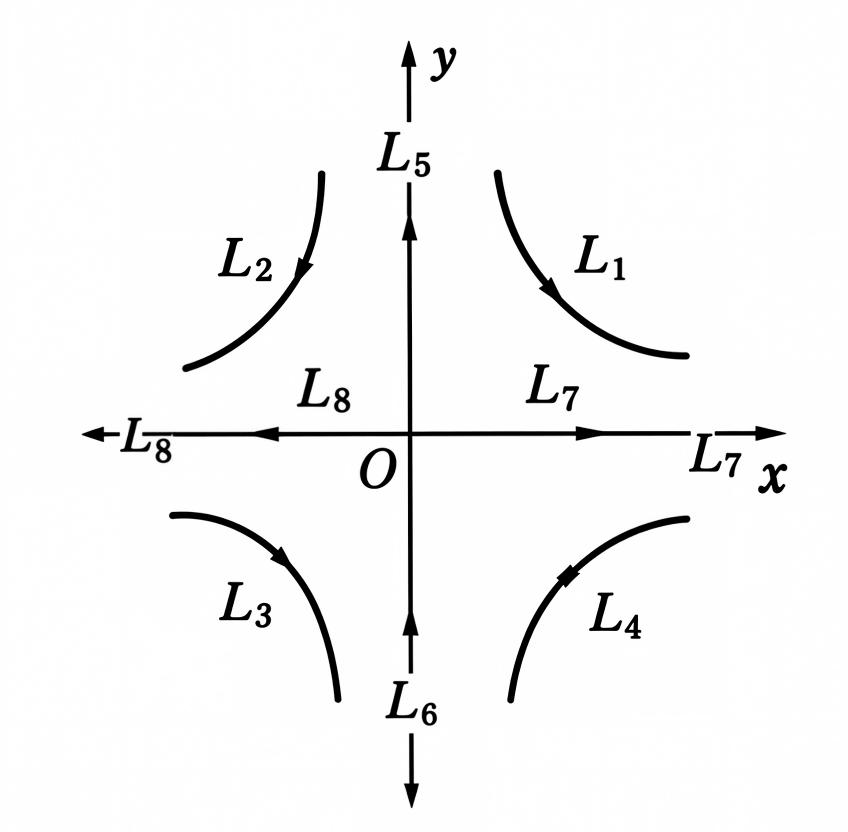
\includegraphics[width=0.5\linewidth]{figure/1.3}
	\captionof{figure}{}
\end{center}
对上图，$L_1, L_2, L_3, L_4$ —— 远离轨线；$L_5, L_6$ —— 正向渐近, 负向远离轨线；$L_7, L_8$ —— 负向渐近, 正向远离轨线；$O$ —— $P$ 稳定轨线.

\begin{center}
	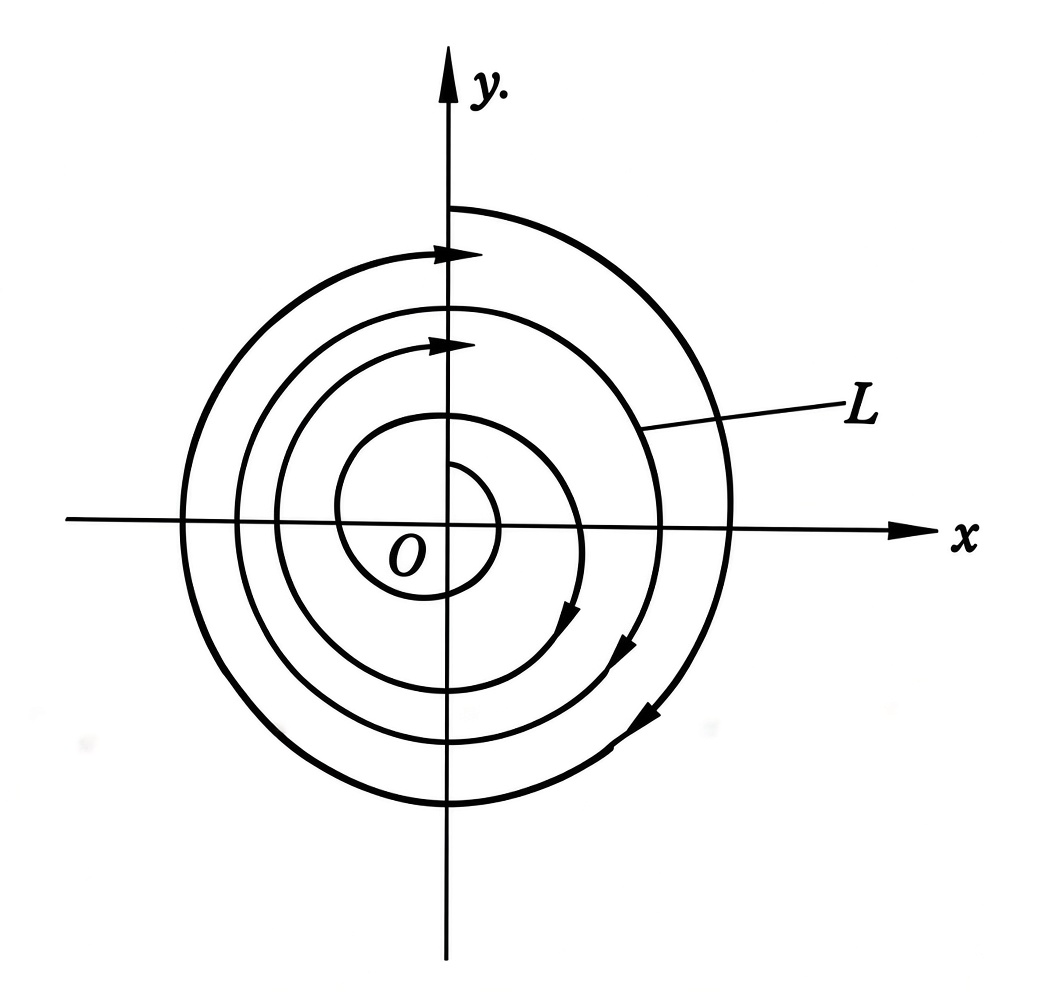
\includegraphics[width=0.5\linewidth]{figure/1.4}
	\captionof{figure}{}
\end{center}
原点 $O$ 和闭轨线 $L$ ($r = 1$) —— $P$ 式稳定轨线；$L_r(0 < r < 1)$ —— 渐近轨线；$L_r(r > 1)$ —— 正向渐近, 负向远离轨线.

\begin{example}{}{lim-cycle}
给定微分方程
\[
\begin{aligned}
\frac{\dd x}{\dd t} &= y + x[1 - (x^2 + y^2)], \\
\frac{\dd y}{\dd t} &= -x + y[1 - (x^2 + y^2)].
\end{aligned}
\]
令 $x = r\cos\theta, y = r\sin\theta$，原方程化为
\[
\frac{\dd r}{\dd t} = r(1 - r^2), \quad \frac{\dd \theta}{\dd t} = -1,
\]
或者
\[
\frac{\dd r}{\dd \theta} = r(r^2 - 1).
\]
易知 $r = 0, r = 1$ 都是轨线，而且 $\dd \theta/\dd t < 0$ 和 $(r - 1) \dd r/\dd \theta > 0$. 故在相平面 $(x, y)$ 上的图形如图~1.4.
\end{example}

% ============================================================
%  §4  平面上的动力系统
% ============================================================
\sourceSection{平面上的动力系统}

给定微分方程组
\[
\begin{cases}
\dd x/\dd t = X(x, y), \\
\dd y/\dd t = Y(x, y),
\end{cases} \tag{4.1}\label{eq:4.1}
\]
其中 $X(x, y), Y(x, y)$ 是定义在 $\R^2$ 上的连续函数，并且满足条件，以保证初值问题的解唯一. 由定理~\ref{thm:equiv-system}，可认为 \eqref{eq:4.1} 的每个解的存在区间为 $(-\infty, +\infty)$，故 \eqref{eq:4.1} 在 $\R^2$ 上定义了一个动力系统.

\textbf{Jordan 定理}\quad 任何 $\R^2$ 上的单闭曲线 $L$ 将 $\R^2$ 分成两部分 $-D_1$ 和 $D_2$，且 $D_1$ 内任何一点到 $D_2$ 内任何一点的连续路径必与 $L$ 相交.

这一节的结果基本是由解的存在唯一性和 Jordan 定理这个简单的几何事实推得的，其中主要结果是由 H. Poincaré 和 I. Bendixson 得到的. 另外必须指出有些结论只是在底空间是欧氏平面 $\R^2$ 或者二维球面 $S^2$ 时才成立，这主要是因为 Jordan 定理的缘故.

\begin{theorem}{}{closed-sing}
方程 \eqref{eq:4.1} 的所有奇点组成闭集.
\end{theorem}

\begin{proof}
要证，如果 $(x_n, y_n)$ 是奇点，且当 $n \to +\infty$ 时 $(x_n, y_n) \to (\bar x, \bar y)$，则 $(\bar x, \bar y)$ 也是奇点. 由 $X^2(x_n, y_n) + Y^2(x_n, y_n) = 0$，便知
\[
\lim_{n \to +\infty} \left[X^2(x_n, y_n) + Y^2(x_n, y_n)\right] = X^2(\bar x, \bar y) + Y^2(\bar x, \bar y) = 0.
\]
\end{proof}

\begin{definition}{}{non-tangent}
$\overline{N_1N_2}$ 为直线. 如果凡是与 $\overline{N_1N_2}$ 相交的轨线，当 $t$ 增加时只能从 $\overline{N_1N_2}$ 的同一侧到另一侧，而且没有轨线与 $\overline{N_1N_2}$ 相切，则 $\overline{N_1N_2}$ 叫做无切线段.
\end{definition}

\begin{lemma}{}{flow-box}
设 $P_0$ 是 \eqref{eq:4.1} 的常点，则存在过 $P_0$ 的无切线段 $\overline{N_1N_2}$，以及曲边长方形 $ABCD$, $AB \parallel \overline{N_1N_2} \parallel DC$, $AD, BC$ 为轨线段，自 $ABCD$ 内任一点出发的轨线，当它向两侧延续时，必分别与 $AB$ 和 $CD$ 各相交一次（从一侧穿过 $\overline{N_1N_2}$）.
\end{lemma}

\begin{proof}
取 $\varepsilon > 0$ 充分小，使 $\overline{S(P_0, \varepsilon)}$ 中不包含奇点. 作过 $P_0(x_0, y_0)$ 点的轨线的法线段 $\overline{N_1N_2}$，其方程为：
\[
Y(x_0, y_0)(y - y_0) + X(x_0, y_0)(x - x_0) = 0.
\]
令
\[
\lambda(x, y) = Y(x_0, y_0)(y - y_0) + X(x_0, y_0)(x - x_0) = C,
\]
它是一组平行于 $\overline{N_1N_2}$ 的直线族. 对这组平行直线族沿着方程组 \eqref{eq:4.1} 所定义的向量场求方向导数，得
\[
\frac{\dd \lambda}{\dd t} = Y(x_0, y_0) Y(x, y) + X(x_0, y_0) X(x, y).
\]
因 $\dd\lambda/\dd t|_{(x_0, y_0)} = Y^2(x_0, y_0) + X^2(x_0, y_0) > 0$，由连续性，存在 $0 < \delta \leq \varepsilon$，使得当 $(x, y) \in S(P_0, \delta)$ 时，也有 $\dd\lambda/\dd t > 0$. 这就是说，\eqref{eq:4.1} 的轨线在 $S(P_0, \delta)$ 中当 $t$ 增加时沿着 $C$ 增加的方向与平行直线族相交. 如图~1.5 所示，取 $\overline{N_1N_2} \subset S(P_0, \delta)$，$\overline{N_1N_2}$ 就是无切线段. 显然，可以作满足引理要求的曲边长方形 $ABCD \subset S(P_0, \delta)$，将它记为 $\square \overline{N_1N_2}$.
\end{proof}

\begin{center}
	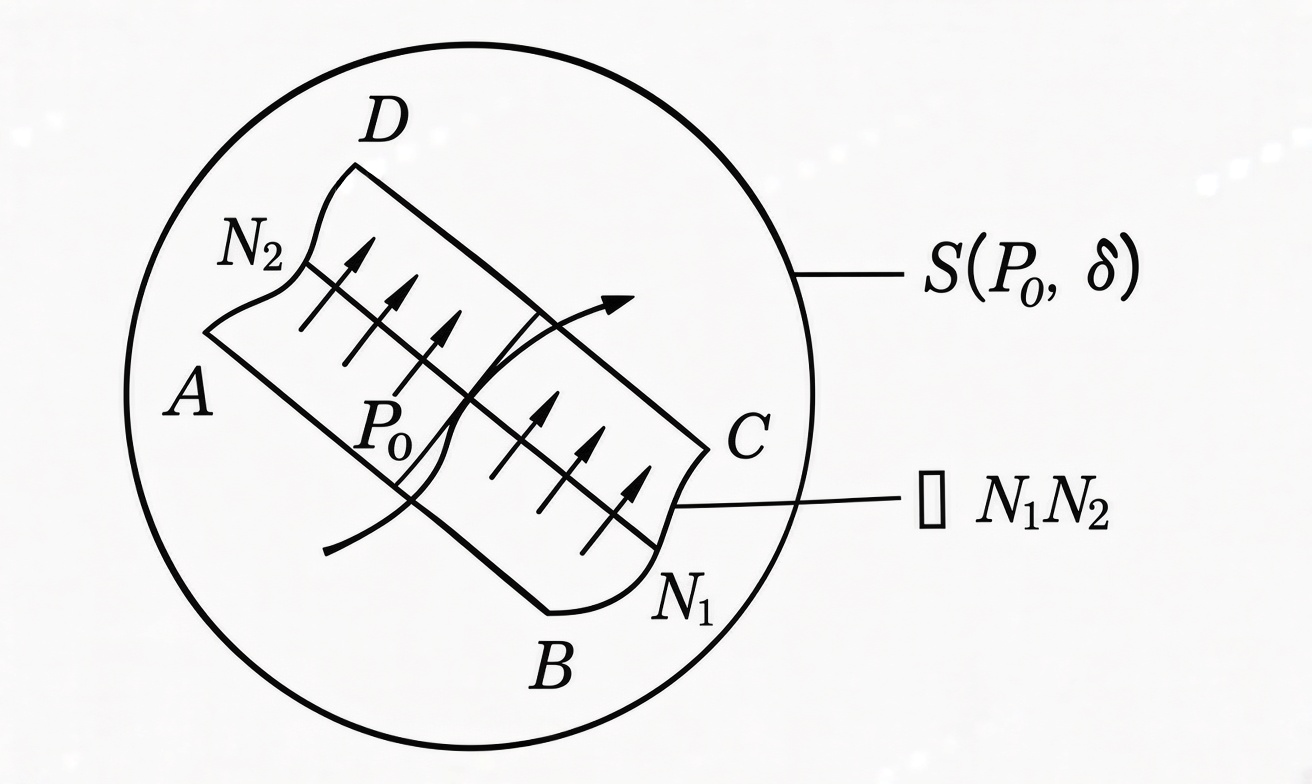
\includegraphics[width=0.5\linewidth]{figure/1.5}
	\captionof{figure}{}
\end{center}


在 $\R^n$ 上定义的一个连续向量场，它在 $\R^n$ 上决定一个连续流；在任何常点 $P$ 附近，也能作出具有类似上述性质的曲边长方体，它叫做过 $P$ 点的流盒. 沿用这个名词，我们也将满足引理~\ref{lem:flow-box} 的曲边长方形叫做过 $P$ 点的流盒.

\begin{lemma}{}{order}
设 $\overline{N_1N_2}$ 为无切线段，$\square \overline{N_1N_2}$ 为满足引理~\ref{lem:flow-box} 的流盒，又设 $f(P, I^+)$（或 $f(P, I^-)$）与 $\overline{N_1N_2}$ 按时间次序相交于 $M_1, M_2, M_3$，则 $M_2$ 必落在 $M_1$ 与 $M_3$ 之间.
\end{lemma}

\begin{proof}
只证括号外的. $f(P, I^+)$ 与 $\overline{N_1N_2}$ 相交于 $M_2$ 之后不能离开（或进入）由轨线段 $M_1SM_2$ 与无切线段 $M_1M_2$ 所围成的区域 $D$，如上图中 (1)（或图 (2)）所示. 因根据解的唯一性，$f(P, I^+)$ 不能与 $M_1SM_2$ 相交，也不能经过 $M_1M_2$ 离开（或进入）$D$. 既然 $f(P, I^+)$ 自 $M_2$ 之后永远停留在 $D$ 内（或外），$M_3$ 就不能落在 $M_1, M_2$ 之间，而 $M_2$ 必落在 $M_1$ 与 $M_3$ 之间. 这时我们简称 $f(P, I^+)$ 按次序与无切线段 $\overline{N_1N_2}$ 相交于 $M_1, M_2, M_3$.
\end{proof}

\begin{theorem}{}{poincare}
设 $f(P, I)$ 是 $P^+$（或 $P^-$）稳定轨线，则 $f(P, I)$ 是奇点或闭轨线.
\end{theorem}
\begin{center}
	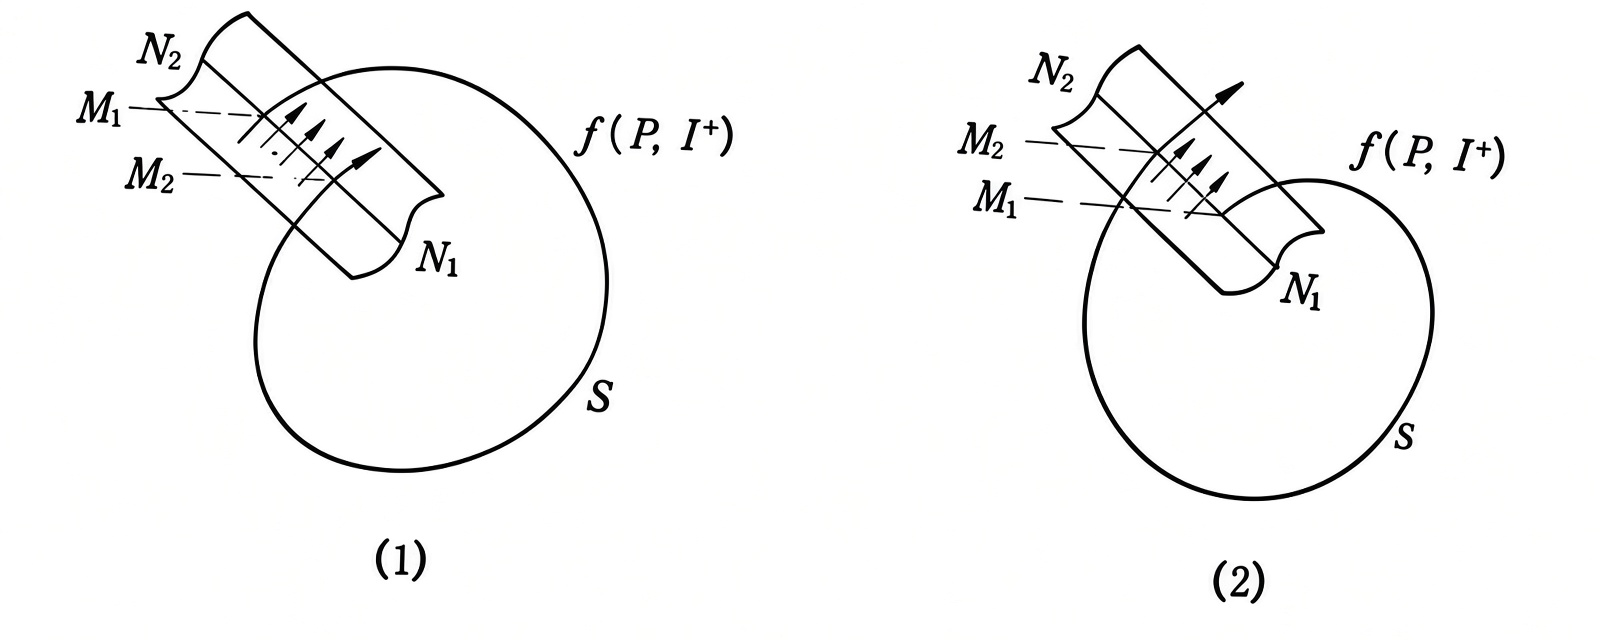
\includegraphics[width=0.7\linewidth]{figure/1.6}
	\captionof{figure}{}
\end{center}

\begin{proof}
只证正向的情形. 因 $\Omega_P \cap f(P, I^+) \neq \emptyset$，取 $M_1 \in \Omega_P \cap f(P, I^+)$. 如 $M_1$ 是奇点，则 $f(P, I^+) = \Omega_P = M_1$，定理得证. 如 $M_1$ 不是奇点，过 $M_1$ 作流盒 $\square \overline{N_1N_2}$. 因 $M_1 \in \Omega_P$，必存在 $T > 0$, $f(P, I^+)$ 离开 $\square \overline{N_1N_2}$ 后，在时刻 $T$ 时，再次进入 $\square \overline{N_1N_2}$，即 $f(P, T) \in \square \overline{N_1N_2}$. 根据 $\square \overline{N_1N_2}$ 的性质，$f(P, I^+)$ 在 $T$ 附近向正向或负向延续时，与 $\overline{N_1N_2}$ 相交于 $M_2$，其图形只能是下列三种情形之一：图~1.6 中的 (1), (2) 或下图~1.7. 如发生图~1.6 中的情形 (1) 或 (2)，由引理~\ref{lem:order}, $f(P, I^+)$ 自 $M_2$ 之后不可能再回到 $M_1$ 的任意小邻域. 故 $M_1 \in \Omega_P$，得矛盾. 故只能是图~1.7 的情形，即 $f(P, I) = L_P$ 是闭轨线.
\end{proof}


\begin{corollary}{}{pplus-pp}
平面上的 $P^+$ 或 $P^-$ 稳定轨线必为 $P$ 式稳定轨线.
\end{corollary}

本定理说明，在 $\R^2$ 上的 $P$ 式稳定轨线只能是奇点或闭轨线. 但当底空间不是 $\R^2$ 时，一般来说，$P$ 式稳定轨线可以是非常复杂的，它不属于本节讨论的范围.
\begin{center}
	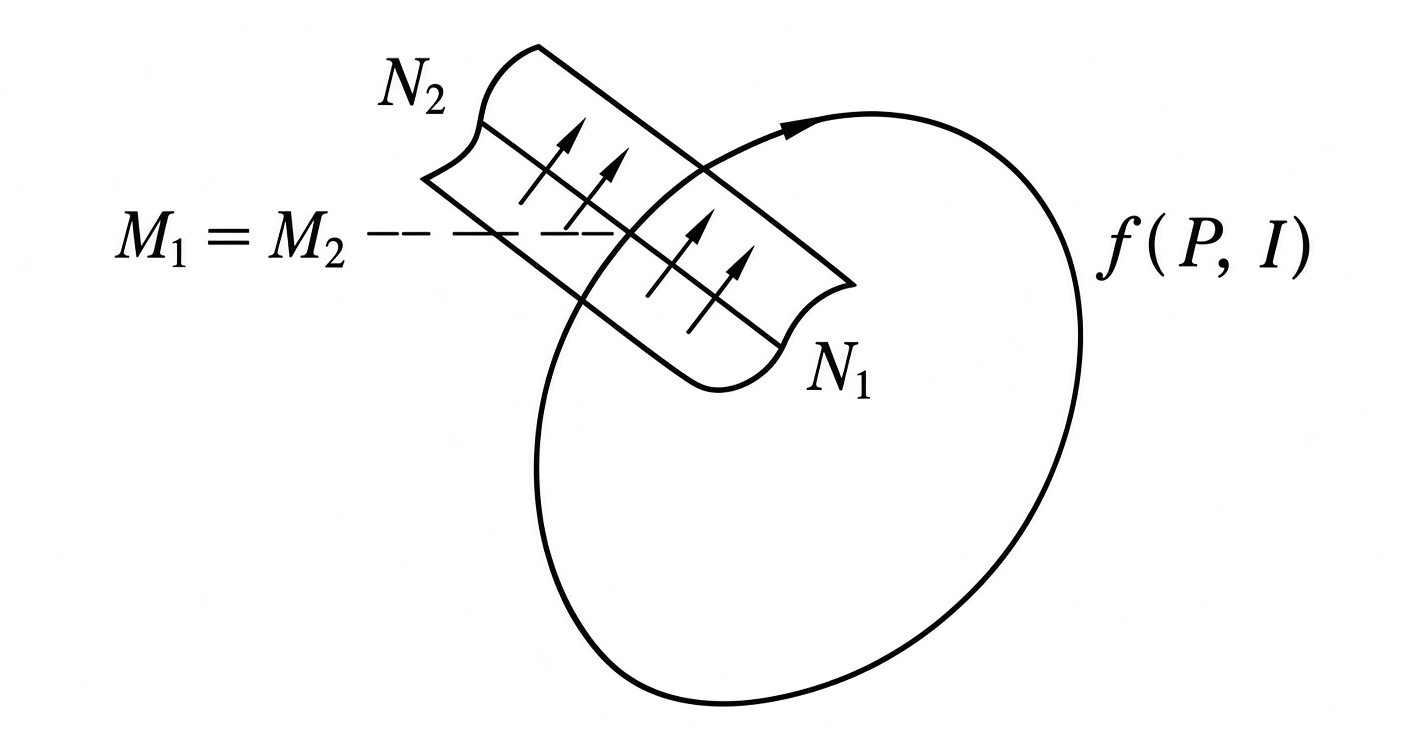
\includegraphics[width=0.7\linewidth]{figure/1.7}
	\captionof{figure}{}
\end{center}

\begin{theorem}{}{omega-L}
如 $L$ 为闭轨线，$L \subset \Omega_P(A_P)$，则 $\Omega_P = L$ ($A_P = L$).
\end{theorem}

\begin{proof}
只证括号外的. 要证，对任意小的 $\varepsilon_1 > 0$，存在充分大的实数 $r > 0$, $f(P, t) \subset S(L, \varepsilon_1)$，当 $t > r$ 时，这就证明了 $\Omega_P = L$. 如图~1.8 所示，在 $L$ 上取一点 $Q$，过 $Q$ 作流盒 $\square \overline{N_1N_2} \subset S(Q, \varepsilon_1)$. 取 $\varepsilon_2$ 充分小，使 $S(Q, \varepsilon_2) \subset \square \overline{N_1N_2}$. 设 $T$ 为 $L$ 的周期. 根据解对初值的连续性，对 $\varepsilon_2$ 与 $T$，存在正数 $\delta(\varepsilon_2, T) < \varepsilon_2$，当 $\rho(Q, R) < \delta$ 和 $0 \leq t \leq T$，就有 $\rho(f(Q, t), f(R, t)) < \varepsilon_2$. 因 $Q \in \Omega_P$，存在 $f(P, t_1) = M_1 \in S(Q, \delta) \cap \overline{N_1N_2}$，故有 $\rho(f(P, t_1 + t), f(Q, t)) < \varepsilon_2$, $0 \leq t \leq T$，即 $\rho(f(P, t_1 + T), Q) < \varepsilon_2$，即 $f(P, t_1 + T) \in S(Q, \varepsilon_2) \subset \square \overline{N_1N_2}$. 由 $\square \overline{N_1N_2}$ 的性质，当 $f(P, t_1 + T)$ 向正向或负向延长时必与 $\overline{N_1N_2}$ 相交，设交点为 $M_2$. 由引理~\ref{lem:order}, $M_2$ 必落在 $M_1$ 与 $Q$ 之间. 否则 $Q$ 将不属于 $\Omega_P$，故 $\rho(M_2, Q) < \delta$. 再由 $\delta$ 的定义及 $\square \overline{N_1N_2}$ 的性质，$f(P, t)$ 自 $M_2$ 之后都落在 $S(L, \varepsilon_2)$ 中. 因 $\varepsilon_1$ 为任给，故 $\Omega_P = L$.
\end{proof}
\begin{center}
	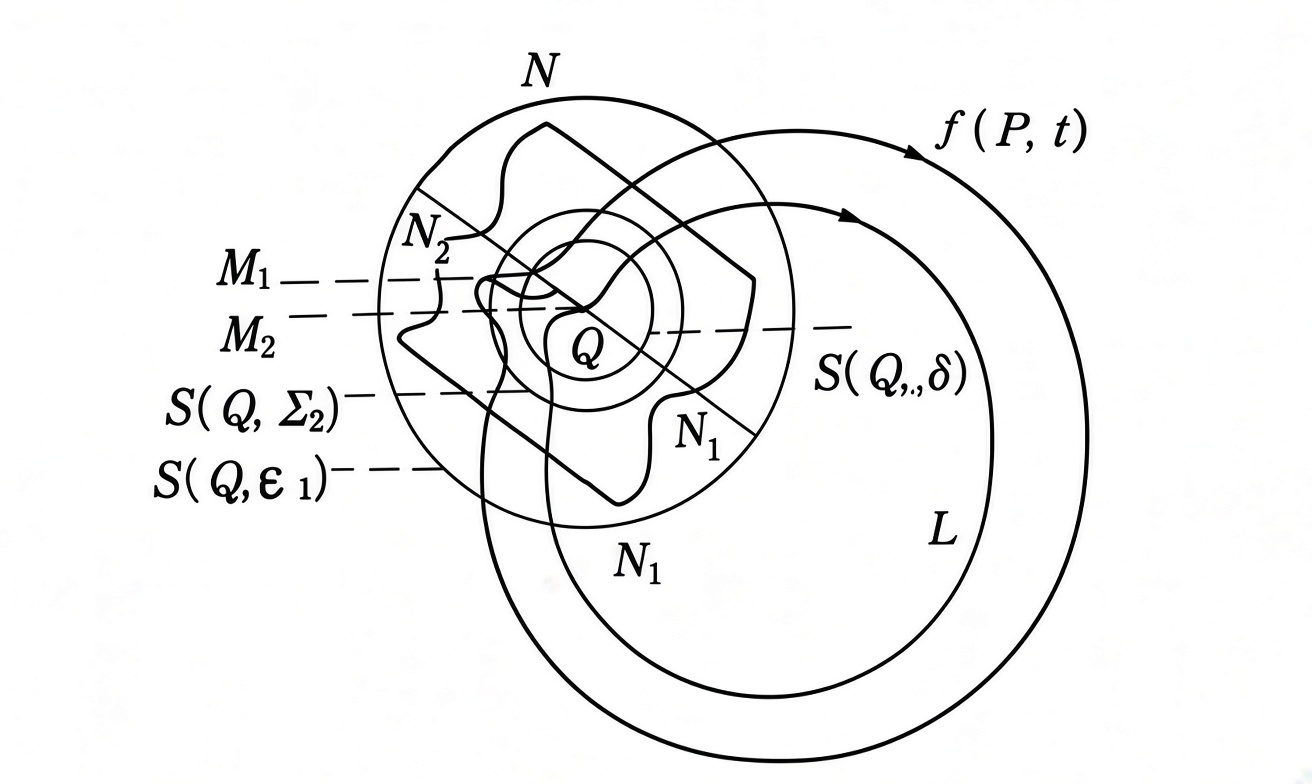
\includegraphics[width=0.7\linewidth]{figure/1.8}
	\captionof{figure}{}
\end{center}



\begin{theorem}{}{omega-bounded}
若 $\Omega_P(A_P)$ 有界非空，且不包含奇点，则 $\Omega_P(A_P)$ 必为闭轨线.
\end{theorem}

\begin{proof}
只证括号外的. 若 $f(P, I)$ 为 $P^+$ 稳定轨线，则由定理~\ref{thm:poincare}, $f(P, I) = \Omega_P$ 为闭轨线，本定理成立. 若 $f(P, I)$ 非 $P^+$ 稳定轨线，即 $f(P, I^+) \cap \Omega_P = \emptyset$. 则可用反证法. 设 $\Omega_P$ 非闭轨线，取 $Q \in \Omega_P$，因 $\Omega_P$ 有界，故 $\Omega_P$ 非空，且 $\Omega_P \subset \Omega_P$，根据定理~\ref{thm:omega-L}, $\Omega_P$ 非闭轨线，否则 $\Omega_P = L$ 将为闭轨线. $\Omega_P$ 非奇点又非闭轨线，由定理~\ref{thm:poincare}, $f(Q, I^+)$ 非 $P^+$ 稳定，即 $f(Q, I^+) \cap \Omega_P = \emptyset$. 取 $B \in \Omega_P$，因 $B$ 非奇点，过 $B$ 作流盒 $\square \overline{N_1N_2}$. 因 $B \in f(Q, I^+)$，故存在时间序列 $t_1 < t_2 < t_3$, $M_i = f(Q, t_i) \in \overline{N_1N_2}$, $i = 1, 2, 3$.
\[
\rho(M_1, B) > \rho(M_2, B) > \rho(M_3, B) > 0.
\]
取 $\delta > 0$ 充分小，使得
\[
S(M_i, \delta) \cap S(M_j, \delta) = \emptyset, \quad i, j = 1, 2, 3, i \neq j.
\]
\[
S(M_i, \delta) \subset \square \overline{N_1N_2}, \quad i = 1, 2, 3.
\]
因 $M_3 \in \Omega_P$，由 $\square \overline{N_1N_2}$ 的性质，存在 $R = f(P, T) \in \overline{N_1N_2} \cap S(M_3, \delta)$. 根据图~1.9 (1)（或 (2)），当 $t > T$, $f(P, t)$ 将不可能进入（或离开）由轨线弧 $M_3SM_3$ 及无切线段 $M_1M_3$ 所围成的区域，因此不可能进入 $S(M_1, \delta)$. 故 $M_1 \in \Omega_P$，得矛盾，这就否定了反证法的前提，定理得证.
\end{proof}
\begin{center}
	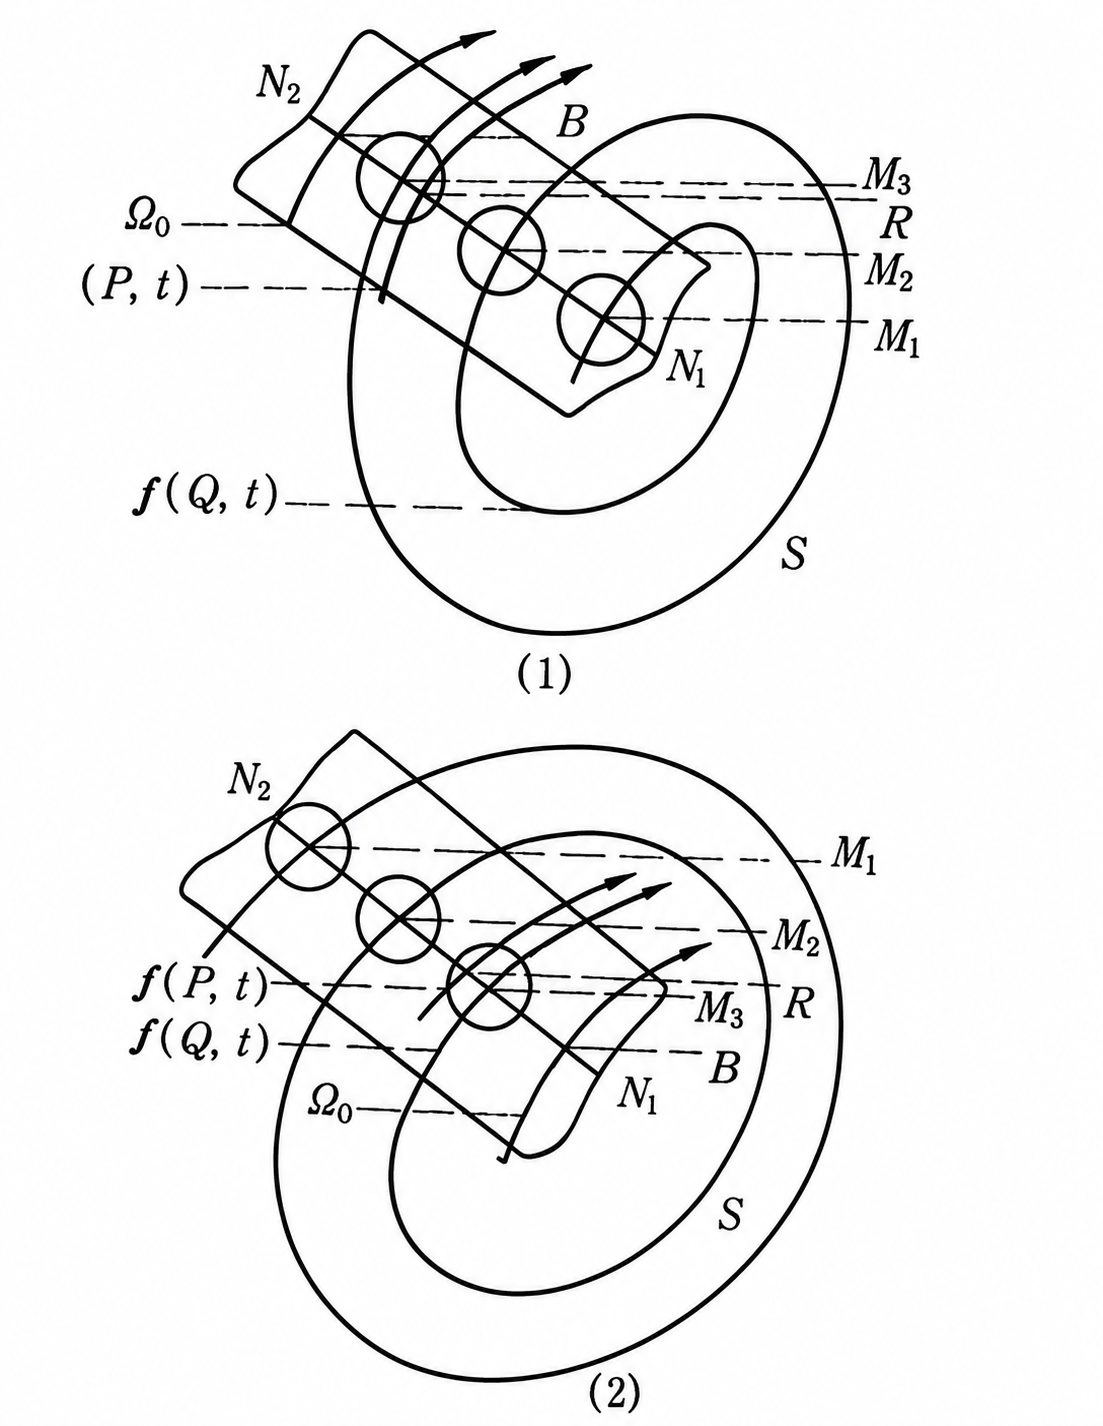
\includegraphics[width=0.5\linewidth]{figure/1.9}
	\captionof{figure}{}
\end{center}


注意，定理中关于 $\Omega_P$ 有界的条件是不可缺少的，否则 $\Omega_P$ 可以既不包含奇点，也非闭轨线. 请看下图.
\begin{center}
	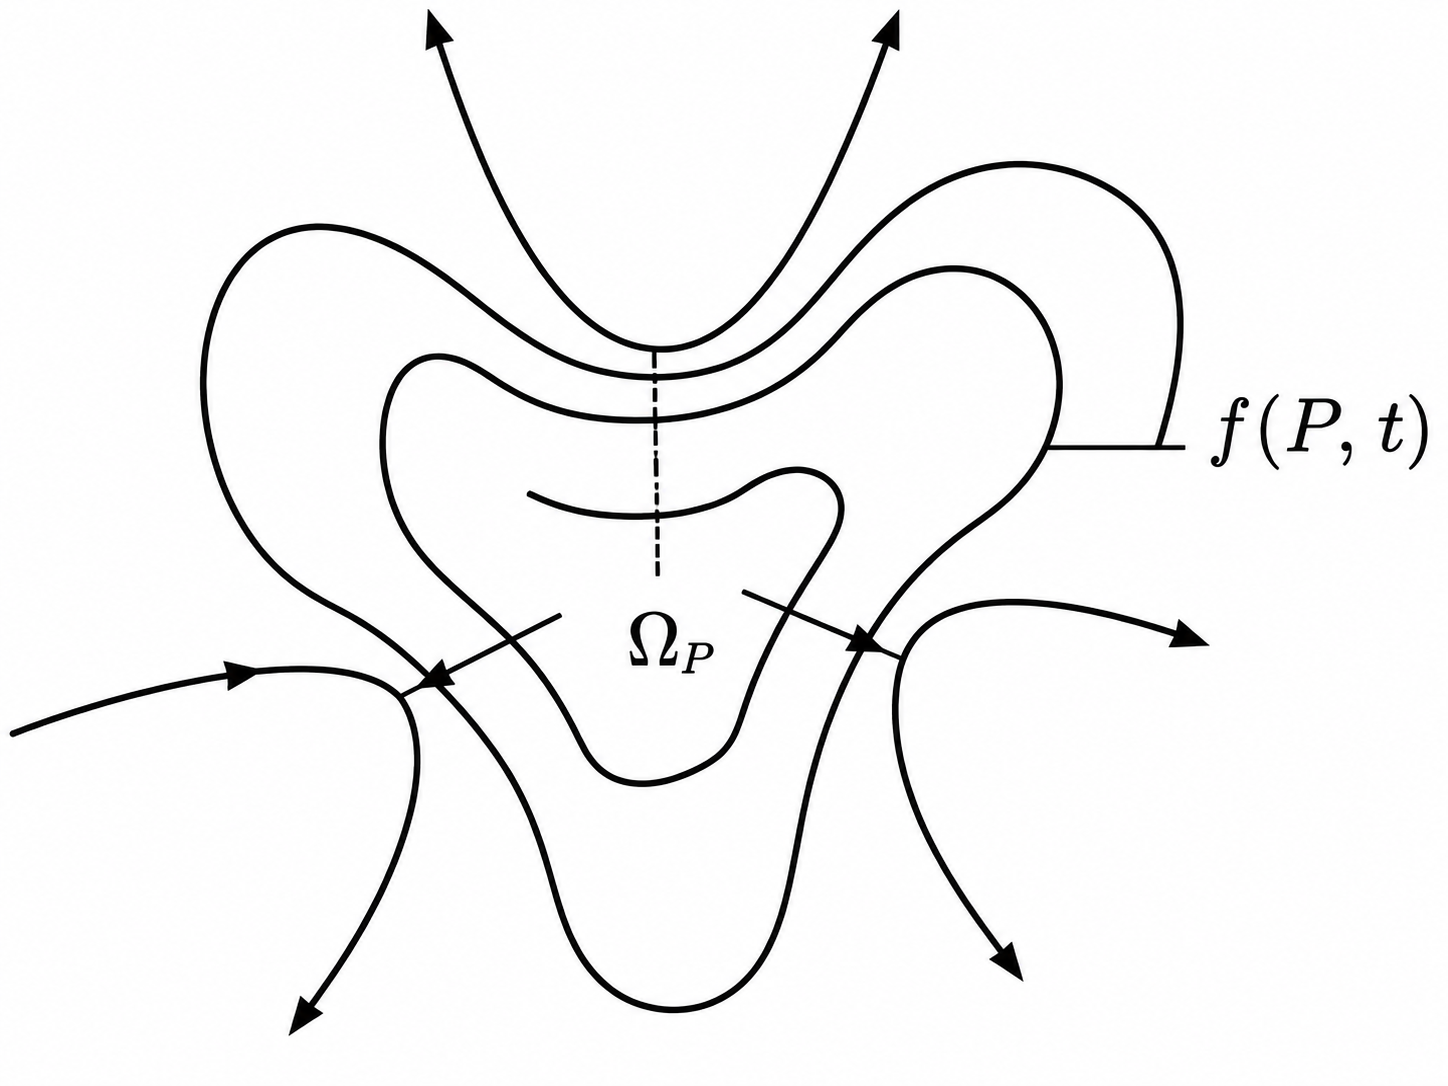
\includegraphics[width=0.5\linewidth]{figure/1.10}
	\captionof{figure}{}
\end{center}
\newpage


\begin{theorem}{}{omega-neighbor}
若 $f(P, I)$ 非闭轨线，$\Omega_P$ 为闭轨线，则存在 $S(P, \varepsilon)$，对任何 $Q \in S(P, \varepsilon)$，必有 $\Omega_Q = \Omega_P$.
\end{theorem}

由定理~\ref{thm:omega-bounded} 及解对初值的连续依赖性便可证明.

\begin{corollary}{}{ap-omega}
若 $f(P, I)$ 非闭轨线，$\Omega_P$ 为闭轨线，则 $A_P \cap \Omega_P = \emptyset$.
\end{corollary}

\begin{theorem}{}{sing-inside}
在平面上任何闭轨线 $L$ 所包围的区域中必有奇点.
\end{theorem}

\begin{proof}
令 $L$ 所包围的区域为 $D$. 假设 $D$ 中无奇点. 任取 $P_1 \in D$，由定理~\ref{thm:omega-bounded}, $\Omega_{P_1}$ 和 $A_{P_1}$ 均为闭轨线. 由定理~\ref{thm:omega-neighbor} 的推论，或者 $L_{P_1} = \Omega_{P_1} = A_{P_1}$ 是闭轨线，或者 $\Omega_{P_1} \neq A_{P_1}$，也即在 $D$ 中必有异于 $L$ 的闭轨线 $L_1 \subset L$（符号 $L_1 \subset L$ 的意思是 $L_1 \subset D$）. 同样可证存在异于 $L_1$ 的闭轨线 $L_2 \subset L_1 \subset L$. 对任意点 $Q(x, y) \in D$，定义函数
\[
F(x, y) = \begin{cases}
d, & \text{当 } f(Q, I) \text{ 非闭轨线}, d \text{ 为 } D \text{ 的面积}, \\
a(x, y), & \text{当 } f(Q, I) \text{ 是闭轨线}, a(x, y) \text{ 是 } f(Q, I) \text{ 所包围的面积}.
\end{cases}
\]
$F(x, y) > 0$ 为 $D$ 上的单值函数，故 $F(x, y)$ 在 $D$ 上有下确界 $C < d$，因 $F(x, y)$ 不一定连续，故 $F(x, y)$ 不一定达到下确界，但必存在 $(x_n, y_n) \in D$，使 $F(x_n, y_n) \to C$. 因 $(x_n, y_n)$ 有界，必有收敛子序列. 为符号简单起见，就设 $(x_n, y_n) \to (x_0, y_0)$, $A(x_0, y_0) \in D$. 考虑轨线 $f(A, I)$. 设 $f(A, I)$ 非闭轨线，由定理~\ref{thm:omega-bounded}, $\Omega_A$ 为闭轨线. 由定理~\ref{thm:omega-neighbor}，存在 $S(A, \varepsilon) \subset D$，对任何 $B \in S(A, \varepsilon)$, $f(B, I)$ 非闭轨线. 且 $\Omega_B = \Omega_A$. 故由定理定义，$F(x, y) = d$，当 $(x, y) \in S(A, \varepsilon)$，得矛盾. 故 $f(A, I) = L_A$ 为闭轨线. 于是存在闭轨线 $L'$ 和 $L''$, $L'' \subset L' \subset L_A$. 对充分小的 $\varepsilon > 0$ 及 $Q(x, y) \in S(A, \varepsilon)$，考虑 $f(Q, I)$. 如果 $f(Q, I)$ 为闭轨线，则 $L'' \subset L' \subset L_Q = f(Q, I)$. 设 $d'$ 和 $d''$ 分别是 $L'$ 和 $L''$ 所包围的区域的面积，则 $F(x, y) > d' > d''$；如果 $L_A$ 非闭轨线，则按定义 $F(x, y) = d$，故对一切 $(x_n, y_n) \in S(A, \varepsilon)$, $F(x_n, y_n) > d' > d''$. $\lim F(x_n, y_n) = C \geq d' > d''$. 这与 $F(x, y)$ 在 $D$ 上的下确界为 $C$ 相矛盾. 因而 $L_A$ 既不能是闭轨线，也不能是非闭轨线. 这就推翻了 $D$ 中无奇点的假设，定理得证.
\end{proof}

本定理也可用超限归纳法来证明，请参看文献~\cite{petrovskii-stepanov-1949} 中第二章.

\begin{theorem}{(Poincaré-Bendixson 环域定理)}{poincare-bendixson}
设 $D$ 是由两条单闭曲线 $L_1$ 和 $L_2$ 所包围成的环域，并且在 $D$ 内无奇点；又设当 $t$ 增加时从 $L_1, L_2$ 上出发的轨线都进入（或都离开）$D$，则在 $D$ 内存在闭轨线 $L$，其相对位置是 $L_1 \subset L \subset L_2$.
\end{theorem}

\begin{proof}
由定理~\ref{thm:omega-bounded}，在 $D$ 内有闭轨线 $L$. 由定理~\ref{thm:sing-inside}，其相对位置必为 $L_1 \subset L \subset L_2$.
\end{proof}

本定理的条件可减弱成：$\bar D$ 上无奇点，从 $L_1$ 和 $L_2$ 上出发的轨线都不能离开（或都不能进入）$\bar D$，但 $L_1$ 和 $L_2$ 上均有奇点，从它出发的轨线进入（或离开）$D$，则 $D$ 内有闭轨线. 换句话说，环域 $D$ 的内外境界线 $L_1$ 和 $L_2$ 都可以包含轨线弧.

以下讨论闭轨线附近轨线的分布情形.

\begin{theorem}{}{closed-nearby}
设 $L$ 为闭轨线，则对充分小 $\varepsilon > 0$，存在相应适当小 $\delta > 0$，对任何 $Q \in S(L, \delta)$，至少 $f(Q, I^+), f(Q, I^-)$ 之一落在 $S(L, \varepsilon)$ 中，并且与过 $L$ 上每一点的无切线段按同一顺序相交（顺时针或逆时针）.
\end{theorem}

\begin{proof}
对任何 $P \in L$，作法线 $\overline{N_1N_2}(P)$. 对任何充分小实数 $\varepsilon_1 > 0$，使 $S(L, \varepsilon_1)$ 中无奇点，并作流盒 $\square \overline{N_1N_2}(P) \subset S(P, \varepsilon_1)$. 令 $\square N_1N_2(P)$ 表示流盒 $\square \overline{N_1N_2}(P)$ 的内点集，它是开集. 由 $L$ 的紧致性，必存在有限个 $\square N_1N_2(P_k)$ 将 $L$ 覆盖住. 即
\[
\bigcup_{k=1}^n \square N_1N_2(P_k) \supset L.
\]
于是便存在充分小 $\varepsilon_2 > 0$，有
\[
S(L, \varepsilon_2) \subset \bigcup_{k=1}^n \square N_1N_2(P_k).
\]
设点 $P_1, P_2, \cdots, P_k, \cdots, P_n, P_1$ 按顺序两两相邻地排列在 $L$ 上. 设 $T$ 为 $L$ 的周期. 由解对初值的连续依赖性，$\exists \delta(\varepsilon_2, T) > 0$，对任何点 $P \in L$，当 $Q \in S(P, \delta)$，与定理~\ref{thm:omega-L} 相类似，可证至少 $f(Q, I^+)$ 和 $f(Q, I^-)$ 之一落在 $S(L, \varepsilon_2)$ 中. 由 $L$ 的紧致性，可使这里的 $\delta$ 与 $P$ 无关. 设 $f(Q, I^+)$ 落在 $S(L, \varepsilon_2)$ 中，由向量场的连续性，$f(Q, I^+)$ 将按顺序与流盒 $\bigcup_{k=1}^n [\square N_1N_2(P_k)]$ 相交. $L_Q$ 可为闭轨线. 若 $L_Q$ 非闭轨线，而 $\Omega_Q = L$ 或 $A_Q = L$，我们就相应地称半轨 $L_Q^+$ 或 $L_Q^-$ 绕 $L$ 盘旋.
\end{proof}

\begin{theorem}{}{annulus}
设 $D$ 是由两条闭轨线 $L_1 \subset L_2$ 所围成的环域，$D$ 中无奇点也无其他闭轨线，则对一切 $Q \in D$，必有 $\Omega_Q = L_1$, $A_Q = L_2$（或者 $\Omega_Q = L_2$, $A_Q = L_1$）.
\end{theorem}

从定理~\ref{thm:omega-bounded} 和~\ref{thm:omega-neighbor} 的推论可立刻推得.

设 $L$ 为闭轨线，$P \in L$，过 $P$ 作无切线段 $\overline{R_1PR_2}$, $\rho(R_1, P) = \rho(P, R_2) = \delta$，其中 $\delta$ 满足定理~\ref{thm:closed-nearby} 的要求，设 $R_1$ 落在 $L$ 之外. 令 $F = \{Q \mid Q \in \overline{R_1P}, f(Q, I) \text{ 为闭轨}\}$，现证 $F$ 为闭集. 用反证法. 设 $F$ 非闭集，则必存在 $Q_n \in F, Q_n \to B \in F$，即 $f(B, I)$ 非闭轨. 由定理~\ref{thm:closed-nearby}, $f(B, I^+)$ 和 $f(B, I^-)$ 之一必停留在 $S(L, \varepsilon_1)$ 中，$\varepsilon_1$ 和 $\delta$ 的取法如定理~\ref{thm:closed-nearby}. 由定理~\ref{thm:omega-bounded}, $\Omega_B$ 或 $A_B$ 是闭轨线. 由定理~\ref{thm:omega-neighbor}, $\exists \eta > 0$，对一切 $R \in S(B, \eta)$, $\Omega_B = \Omega_R$ 或 $A_B = A_R$，但 $f(R, I)$ 非闭轨线. 这与 $Q_n \in F, Q_n \to B$ 相矛盾，故 $F$ 是闭集. 于是下列两种情况必居其一：
\begin{enumerate}
\item $P$ 为 $F$ 的孤立点. 这时存在充分小的 $0 < \xi < \eta$，任何 $R \in \overline{R_1P} \cap S(L, \xi)$, $f(R, I)$ 的正半轨或负半轨落在 $S(L, \varepsilon_1)$ 中，并绕 $L$ 盘旋，相应地有 $\Omega_R = L$ 或 $A_R = L$.
\item $P$ 为 $F$ 的聚点. 这时从 $\overline{R_1P} \cap S(L, \xi)$ 出发的轨线，或者都是闭轨线，或者其中既有异于 $L$ 的闭轨线又有非闭轨线.
\end{enumerate}
对 $\overline{PR_2}$ 上的点也可进行类似的讨论.

\begin{definition}{}{limit-cycle}
设 $L$ 是闭轨线. 如果存在 $S(L, \varepsilon)$，对任何 $Q \in S(L, \varepsilon)$，有 $\Omega_Q = L$（这时 $f(Q, I^+)$ 绕 $L$ 盘旋），或者有 $A_Q = L$（这时 $f(Q, I^-)$ 绕 $L$ 盘旋），则 $L$ 叫做极限环.
\end{definition}

由以上讨论知，闭轨线附近轨线分布必为下列五种情形之一：
\begin{enumerate}
\item 稳定极限环. $\exists S(L, \varepsilon)$，对任何 $Q \in S(L, \varepsilon)$，有 $\Omega_Q = L$.
\item 不稳定极限环. $\exists S(L, \varepsilon)$，对任何 $Q \in S(L, \varepsilon)$，有 $A_Q = L$.
\item 半稳定极限环. $\exists S(L, \varepsilon)$，对任何 $Q \in S(L, \varepsilon)$，当 $Q$ 落在 $L$ 的一侧，$\Omega_Q = L$，当 $Q$ 落在 $L$ 的另一侧，$A_Q = L$.
\item 周期环域. $\exists S(L, \varepsilon)$，对任何 $Q \in S(L, \varepsilon)$, $f(Q, I)$ 是闭轨线.
\item 复型极限环. 对任意 $\varepsilon > 0$, $S(L, \varepsilon)$ 中既有异于 $L$ 的闭轨线，又有非闭轨线.
\end{enumerate}
往后我们将证明，对解析向量场，即 \eqref{eq:4.1} 的右侧是解析函数时，第 5 种情形不可能发生.

以下进一步讨论 $\Omega_P(A_P)$ 的构造.

先讨论 $\Omega_P$ 有界的情形.

设 $\Omega_P = \Omega_P^{(1)} \cup \Omega_P^{(2)}$, $\Omega_P^{(1)}$ 为常点集，$\Omega_P^{(2)}$ 为奇点集，已证 $\Omega_P^{(2)}$ 是闭集. $\Omega_P^{(2)} = \bigcup_\alpha C_\alpha$, $C_\alpha \cap C_\beta = \emptyset$，当 $\alpha \neq \beta$, $C_\alpha$ 是 $\Omega_P^{(2)}$ 的连通分支.

\begin{definition}{}{touch}
对任何点 $Q$，如果 $\Omega_Q \subset C_\alpha$（或 $A_Q \subset C_\alpha$），轨线 $f(Q, I)$ 就叫做正向（或负向）接触 $C_\alpha$.
\end{definition}

\begin{theorem}{}{countable}
考虑轨线 $f(P, I)$，设 $\Omega_P$ 有界，$\Omega_P = \Omega_P^{(1)} \cup \Omega_P^{(2)}$, $\Omega_P^{(1)} \neq \emptyset$, $\Omega_P^{(2)} \neq \emptyset$，则 $\Omega_P^{(1)}$ 中的每一条轨线都正向和负向接触 $\Omega_P^{(2)}$ 中的一个连通分支，同时 $\Omega_P^{(1)}$ 由可列条轨线组成.
\end{theorem}

\begin{proof}
因 $\Omega_P^{(1)} \neq \emptyset$, $\Omega_P^{(2)} \neq \emptyset$，由定理~\ref{thm:omega-L}, $\Omega_P^{(1)}$ 中无闭轨线. 设 $R \in \Omega_P^{(1)}$，因 $\Omega_P$ 是闭集，故 $\Omega_R \subset \Omega_P$, $\Omega_R \neq \emptyset$. 与定理~\ref{thm:omega-bounded} 类似的步骤，可证 $\Omega_R$ 中无奇点（见习题~9）. $\Omega_R$ 有界，由定理~\ref{thm:omega-connected}, $\Omega_R$ 连通，故 $\Omega_R \subset C_\alpha$. 同样可证 $A_R \subset C_\beta$（也可能 $C_\alpha = C_\beta$）. 定理的前半部分已证明了. 再证 $\Omega_P^{(1)}$ 由可列条轨线组成.

取 $A \in \Omega_P^{(1)}$，因 $A$ 为常点，过 $A$ 作流盒 $\square \overline{N_1N_2}$，由 $\square \overline{N_1N_2}$ 的性质，$f(P, I)$ 只能交 $\overline{N_1N_2}$ 于 $A$ 的一侧，设交于 $\overline{AN_2}$，并且 $f(P, I)$ 与 $\overline{AN_2}$ 只能按次序相交于 $M_1, M_2, M_3, \cdots, M_n, \cdots$，且 $M_n \to A$. 因此在 $\square N_1N_2$ 中除了 $A_1AA_2 = f(A, I) \cap \square N_1N_2$ 外，再没有 $\Omega_P$ 的其他的点. 取正整数 $m$ 适当大，使 $S(A, 1/m) \subset \square N_1N_2$. 对 $\Omega_P^{(1)}$ 中每条轨线都作相应的圆 $S(A, 1/m)$，这些圆 $S(A, 1/m)$ 互不包含别的圆的圆心. 因 $\Omega_P$ 有界，可使 $\Omega_P^{(1)} \subset G \subset \R^2$，其中 $G$ 为有界区域. 对固定的整数 $m > 0$, $G$ 上互不包含彼此圆心的圆 $S(A, 1/m)$ 的个数为有限个，不同的半径 $1/m$ 最多是可列个，因而 $G$ 上这样的圆 $S(A, 1/m)$ 的个数最多是可列个. 故 $\Omega_P^{(1)}$ 最多由可列条轨线组成.
\end{proof}

\begin{corollary}{}{cor1-4-10}
如果 $\Omega_P$ 有界，$\Omega_P = \Omega_P^{(1)} \cup \Omega_P^{(2)}$, $\Omega_P^{(1)}$ 非空，$\Omega_P^{(2)}$ 只包含一个奇点 $O$，则 $\Omega_P^{(1)}$ 中最多有可列条轨线，每条轨线都正向和负向接触于 $O$，如图~1.11 所示.
\end{corollary}
\begin{center}
	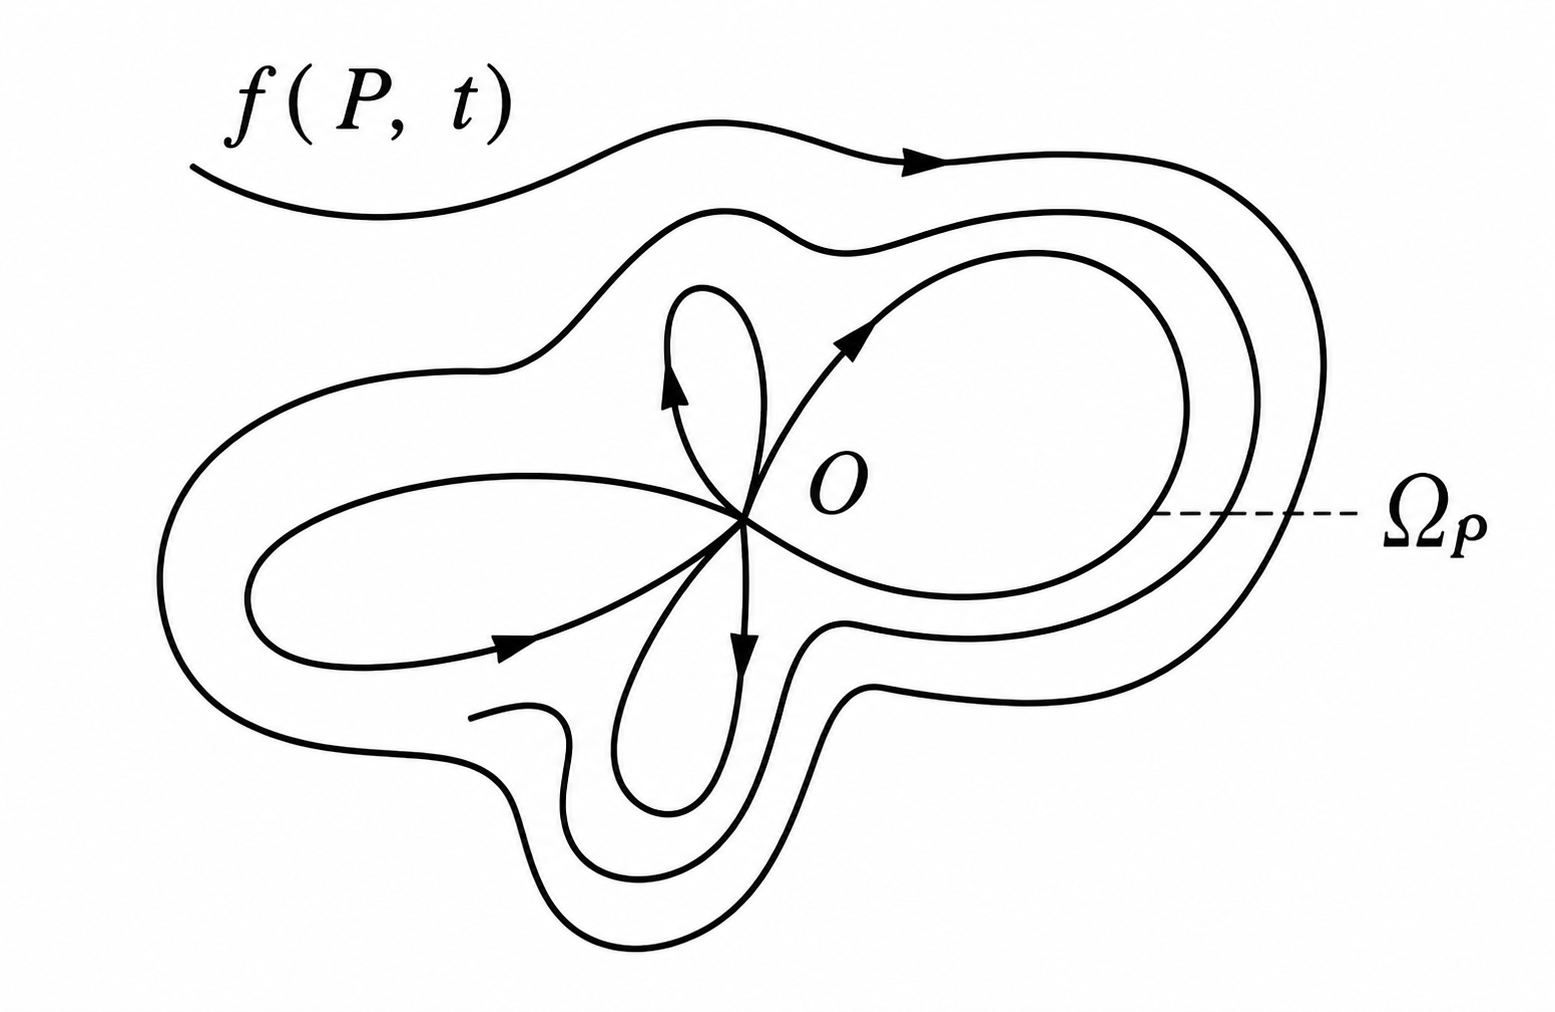
\includegraphics[width=0.5\linewidth]{figure/1.11}
	\captionof{figure}{}
\end{center}


\begin{corollary}{}{cor2-4-10}
$G$ 为有界区域，$G$ 中有唯一的奇点 $O$. 如果 $f(P, I^+) \subset G$，则 $f(P, I^+)$ 必为下列五种情形之一：
\begin{enumerate}
\item[(1)] $P = \{O\}$.
\item[(2)] $\Omega_P = \{O\}, f(P, I^+) \cap \Omega_P = \emptyset$.
\item[(3)] $f(P, I) = \Omega_P$ 为闭轨线，奇点 $O$ 属于 $\Omega_P$ 所包围的区域.
\item[(4)] $\Omega_P$ 为闭轨线，$f(P, I^+) \cap \Omega_P = \emptyset$，奇点 $O$ 属于 $\Omega_P$ 所包围的区域.
\item[(5)] $\Omega_P = \Omega_P^{(1)} \cup \Omega_P^{(2)}, \Omega_P^{(2)} = \{O\}, \Omega_P^{(1)} \neq \emptyset$. 

它们的图形分别如图~1.12 中 (1), (2), (3), (4), (5) 所示. 图形 (4) 中也可能 $f(P, I)$ 落在闭轨线 $\Omega_P$ 所包围的区域中.
\end{enumerate}
\end{corollary}

\begin{center}
	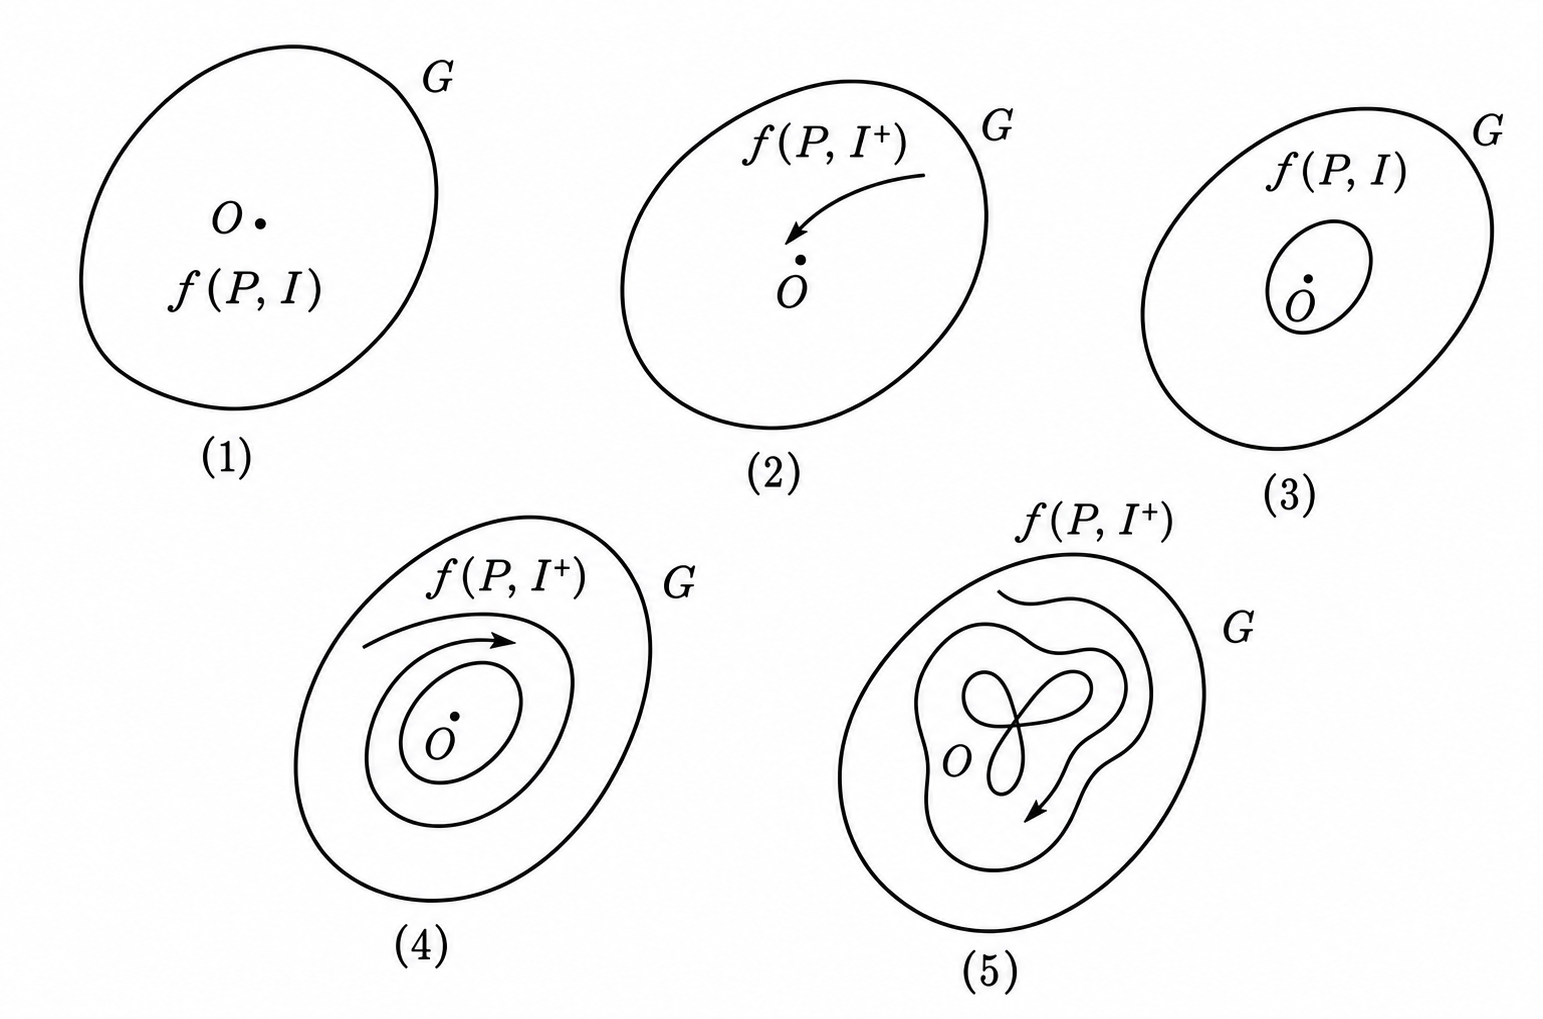
\includegraphics[width=0.7\linewidth]{figure/1.12}
	\captionof{figure}{}
\end{center}
再讨论 $\Omega_P$ 无界的情形.

$S^2$ 是二维球面. $x^*, y^* \in S^2$，定义 $\rho(x^*, y^*)$ 为联接 $x^*$ 和 $y^*$ 的最短球面曲线的长度，于是 $S^2$ 是度量空间. $N$ 是 Euclid 平面的无穷远点. $x^2 + y^2 > r > 0$ 叫做 $N$ 的邻域. $\bar R^2 = \R^2 \cup N$ 叫做将 Euclid 平面封闭化，$\bar R^2$ 是紧致度量空间. 如图所示，$T$ 是测地投影.

\begin{center}
	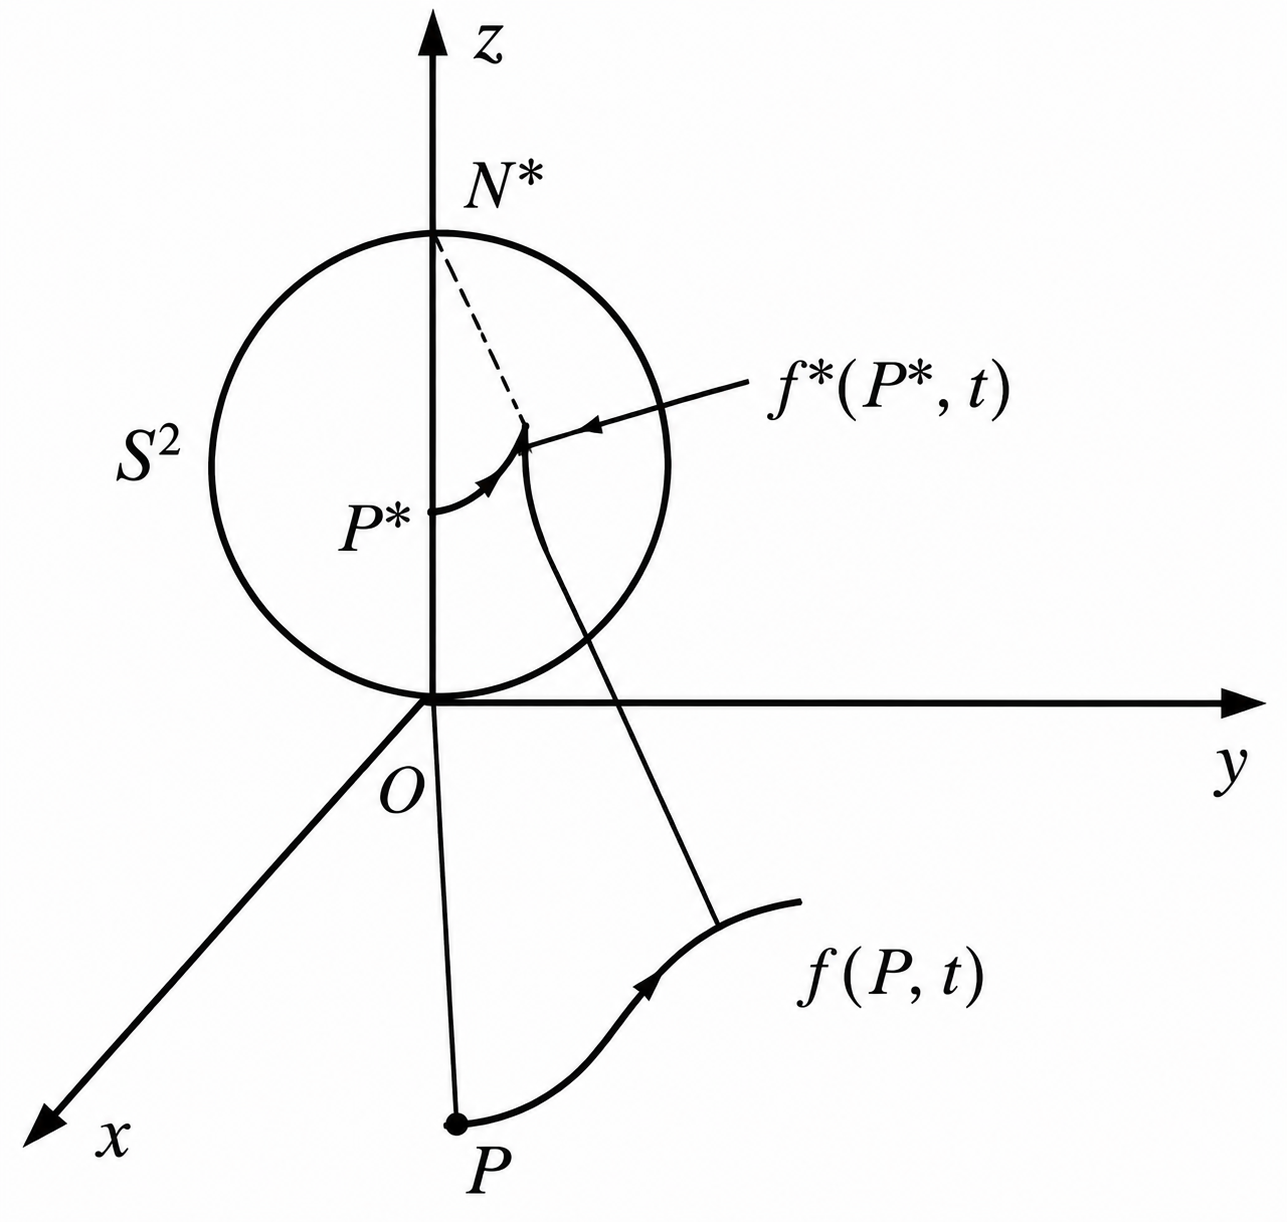
\includegraphics[width=0.5\linewidth]{figure/1.13}
	\captionof{figure}{}
\end{center}

$T: \bar R^2 \to T(\bar R^2) = S^2, N \to T(N) = N^*$. 若 $P \to T(P) = P^*$，定义
\[
f(P, t) \to T(f(P, t)) = f^*(P, t) = \tilde f(P^*, t).
\]
因 $T$ 是拓扑映射，故 $\tilde f(P^*, t)$ 是 $f$ 经过 $T$ 在 $S^2$ 上诱导的动力系统. $\tilde f(N^*, t) = N^*$ 是奇点.

如果 $P_n \to P$，则 $P_n^* \to P^* \neq N^*$；如果 $P_n \to +\infty$，则 $P_n^* \to N^*$. 故若 $\Omega_P$ 有界，则 $\Omega_{P^*} = T(\Omega_P)$；若 $\Omega_P$ 无界，则 $\Omega_{P^*} = T(\Omega_P) \cup N^*$.

\begin{theorem}{}{s2-connected}
$\Omega_{P^*}(A_{P^*})$ 必在 $S^2$ 上连通.
\end{theorem}

\begin{proof}
只证括号外的. 若 $\Omega_P$ 有界，由定理~\ref{thm:omega-connected}, $\Omega_P$ 连通，故 $\Omega_{P^*} = T(\Omega_P)$ 连通. 若 $\Omega_P$ 无界，$\Omega_P \cup N$ 是 $\R^2$ 上的闭集，故 $\Omega_{P^*} = T(\Omega_P) \cup N^*$ 是 $S^2$ 上的闭集. 完全类似定理~\ref{thm:omega-connected} 可证 $S^2$ 上的有界闭集 $\Omega_{P^*}$ 在 $S^2$ 上连通.
\end{proof}

\begin{theorem}{}{unbounded-countable}
如 $\Omega_P$ 无界，$\Omega_P$ 中不包含奇点，则 $\Omega_P$ 至多有可列条无界的轨线组成，而且任何有界区域 $D$ 至多与有限条轨线相交.
\end{theorem}

\begin{proof}
$\Omega_P$ 无界，不包含奇点，故 $\Omega_{P^*} = T(\Omega_P) \cup N^*$, $N^*$ 是 $\Omega_{P^*}$ 中唯一奇点. 类似于定理~\ref{thm:countable} 的推论~1, $\Omega_{P^*}$ 中至多有可列条轨线，每条轨线的正向和负向都接触 $N^*$. 故 $\Omega_P$ 中至多有可列条轨线. 令 $K: x^2 + y^2 \leq r^2$，取 $r$ 充分大，使得 $D \subset K$. 由本节习题 17, $T(\partial K)$ 至多能与 $\Omega_{P^*}$ 中有限条轨线相交，故 $K$ 至多能与 $\Omega_P$ 中有限条轨线相交，故 $D$ 也至多能与 $\Omega_P$ 中有限条轨线相交.
\end{proof}

平面 $\R^2$ 上的区域（连通开集）$D$ 叫做单连通区域，如 $D$ 内任何一条单闭曲线，其内部也属于 $D$.

在平面 $\bar R^2 = \R^2 \cup N$ 上，单连通区域的概念略有不同. $D$ 叫做 $\bar R^2$ 上的单连通区域，如果 $D$ 内任何一条单闭曲线 $l$，或其内部或其外部属于 $D$. 例如平面去掉一点 $P$, $\bar R^2 \setminus \{P\}$ 是 $\bar R^2$ 上的单连通区域，但 $R^2 \setminus \{P\}$ 不是 $R^2$ 上的单连通区域.

$S^2$ 上去掉一点，它是 $S^2$ 上的单连通区域.

在证明下面的定理~\ref{thm:omega-s2-boundary} 之前，我们先举两个例子，来说明单连通区域的边界是连通闭集，它可能是非常复杂的.

\begin{example}{}{sc-region1}
$OBCD$ 是边长为 1 的正方形，正方形内部记成 $K$.
\[
\left.
\begin{aligned}
M_{2k+1}N_{2k+1} &: x = \frac{1}{2^{2k+1}}, \quad 0 \leq y \leq \frac{2}{3}, \\
M_{2(k+1)}M_{2(k+1)} &: x = \frac{1}{2^{2(k+1)}}, \quad \frac{1}{3} \leq y \leq 1,
\end{aligned}
\right\} k = 0, 1, 2, \cdots.
\]
令
\[
G = K \setminus \bigcup_{j=1}^\infty M_jN_j,
\]
$G$ 是单连通区域. 它的边界是
\[
\partial G = \partial K \cup \left(\bigcup_{j=1}^\infty M_jN_j\right).
\]

边界上的点分两类. 一类叫可近边界点，一类叫不可近边界点. $P \in \partial G$ 叫可近边界点，如果存在简单弧段（连续无重点的曲线段）$l \subset G$, $P$ 是 $l$ 的一个端点. $P \in \partial G$ 叫不可近边界点，如果不存在这样的简单弧段. 可近边界点在 $\partial G$ 上处处稠密. 见图~1.14.

在这个例子中，$OD$ 上的点是不可近边界点，其余的边界上的点都是可近边界点. 显然，$\partial G \setminus OD$ 在 $\partial G$ 上处处稠密.
\end{example}
\begin{center}
	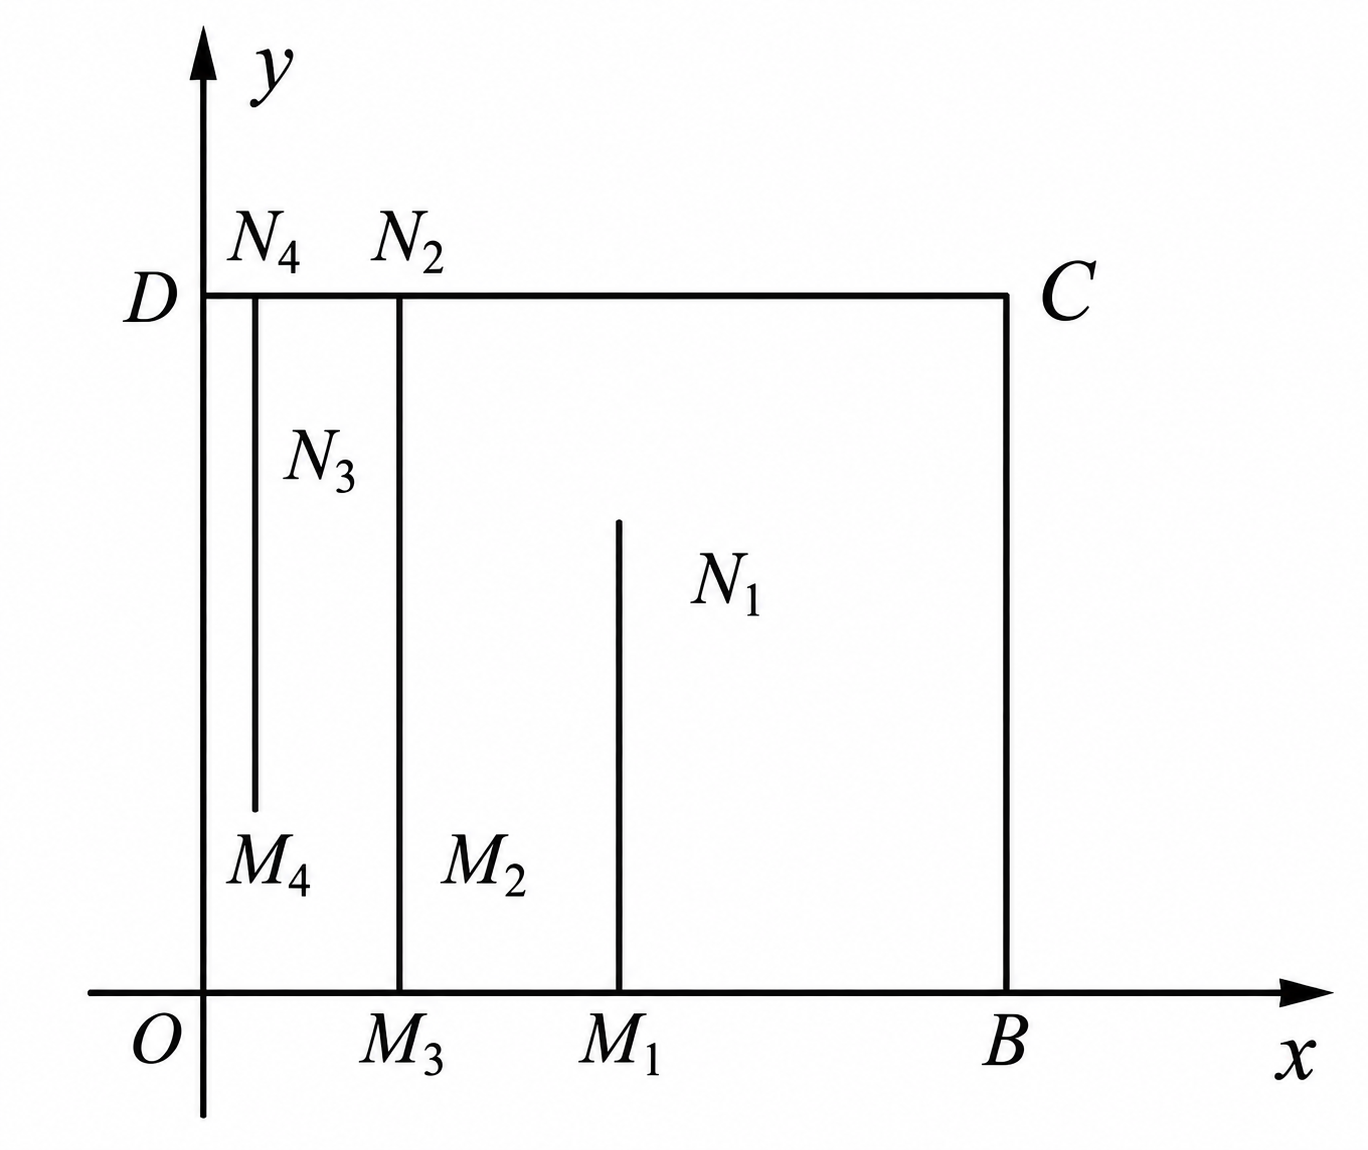
\includegraphics[width=0.4\linewidth]{figure/1.14}
	\captionof{figure}{}
\end{center}


\begin{example}{}{sc-region2}
$K$ 是单位圆的内部. $K$ 内有两个单连通区域 $G_1$ 和 $G_2$，形状都像螺旋线. $G_1$ 是打上阴影的；$G_2$ 是没打阴影的. $G_1$ 和 $G_2$ 有公共的边界.
\[
\partial G_1 = \partial G_2 = L \cup \partial K,
\]
其中 $L$ 是 $G_1$ 和 $G_2$ 的分界.

显然 $L$ 上的点是可近边界点，$\partial K$ 上的点是不可近边界点. $L$ 在 $L \cup \partial K$ 上处处稠密. 见图~1.15.

上例中是两个单连通区域有公共的边界，也可发生更多的单连通区域有公共的边界，这时边界的构造将更加复杂. 请读者参看文献~\cite{aleksandrov-1948} 中的一个有趣的例子.
\end{example}
\begin{center}
	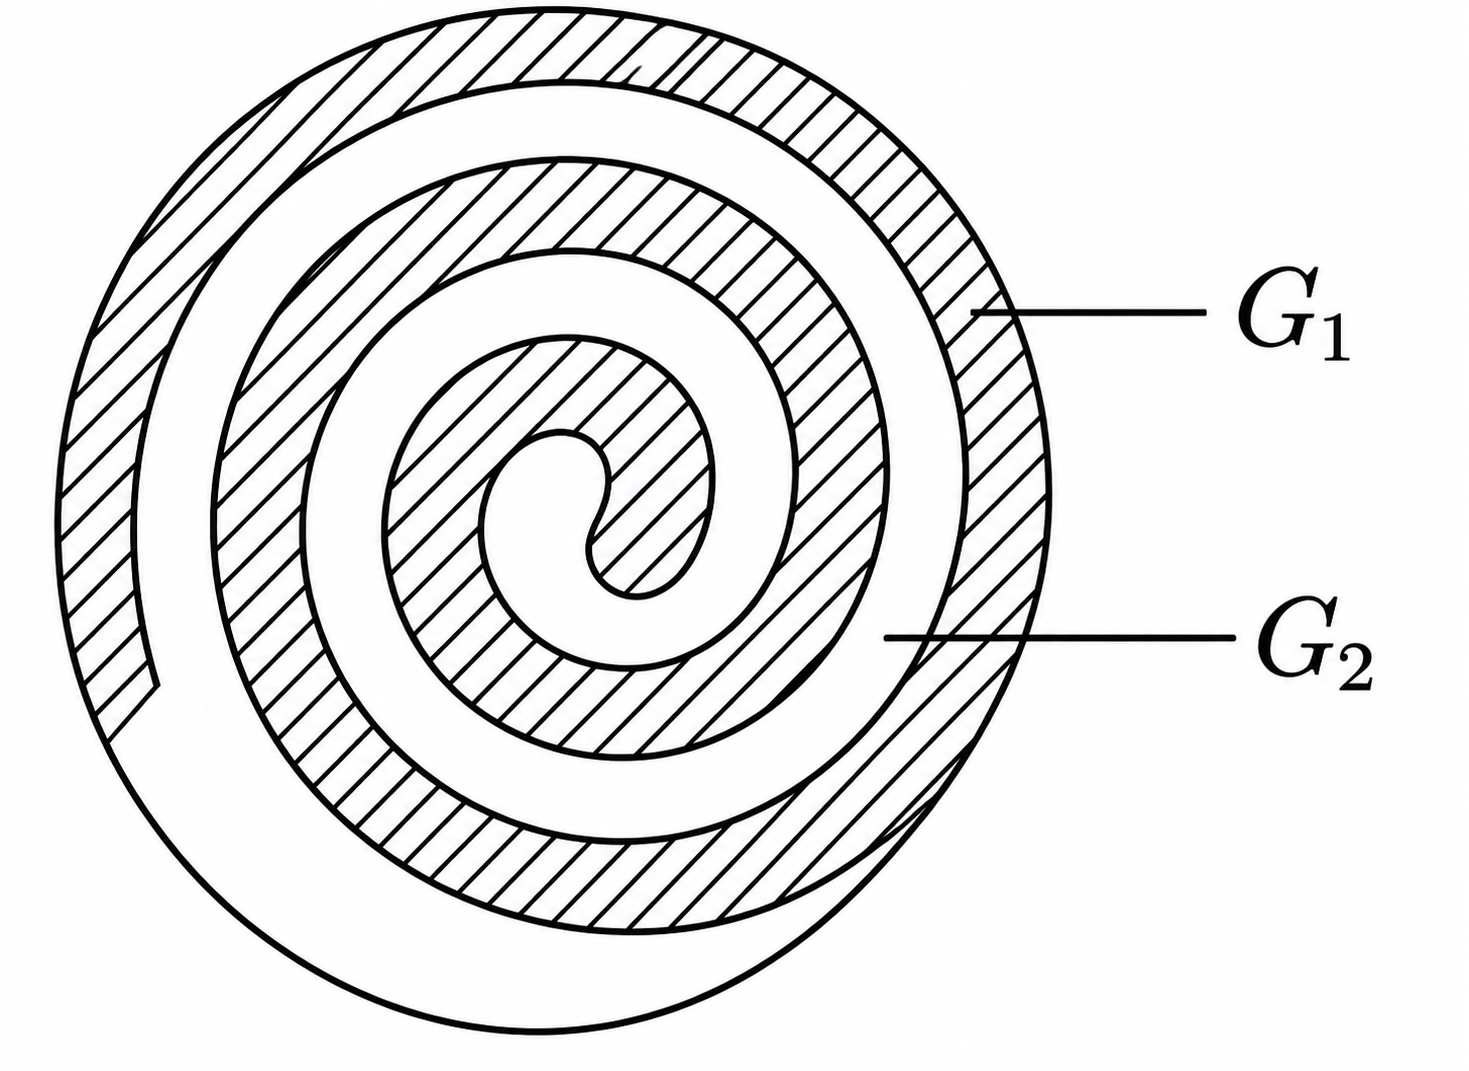
\includegraphics[width=0.4\linewidth]{figure/1.15}
	\captionof{figure}{}
\end{center}

\begin{theorem}{}{omega-s2-boundary}
平面上点集 $E$ 是微分方程所定义的动力系统某一条轨线 $f(P, I)$ 的 $\omega$（或 $\alpha$）极限点集，即 $\Omega_P = E$（或 $A_P = E$），其充要条件为：$T(E) = E^*$ 是 $S^2$ 上单连通区域的边界.
\end{theorem}

\begin{proof}
只证明括号外的情形. 先证必要性.

如果 $\Omega_P \cap f(P, I^+) \neq \emptyset$，则由定理~\ref{thm:poincare}, $E = \Omega_P$ 是奇点或闭轨线，显然 $E^*$ 是 $S^2$ 上单连通区域的边界.

如果 $\Omega_P \cap f(P, I^+) = \emptyset$，则 $\Omega_{P^*} \cap \tilde f(P^*, I^+) = \emptyset$（可能 $N^* \in \Omega_{P^*}$，但 $N^* \notin \tilde f(P^*, I^+)$）. 令 $\Omega_{P^*} = E^*$, $G = S^2 \setminus E^*$. 因 $E^*$ 为闭集，故 $G$ 为开集，$G = \bigcup_\alpha G_\alpha$, $G_\alpha \cap G_\beta = \emptyset$，当 $\alpha \neq \beta$, $G_\alpha$ 为连通分支. 因 $\tilde f(P^*, I^+)$ 连通，$\tilde f(P^*, I) \cap E^* = \emptyset$，故 $\tilde f(P^*, I)$ 必属于其中一个连通分支，设 $\tilde f(P^*, I) \subset G_\alpha$. 于是 $\tilde f(P^*, I)$ 的极限点集 $E^* \subset \bar G_\alpha$，但 $E^* \cap G_\alpha \subset E^* \cap G = \emptyset$，故 $E^* \subset \partial G_\alpha$. 另外 $\partial G_\alpha \subset \partial G = E^*$，故 $E^* = \partial G_\alpha$. 因 $E^*$ 连通，故 $G_\alpha$ 单连通，故 $E^*$ 是单连通区域 $G_\alpha$ 的边界.

现证充分性. 设 $E$ 中只包含一个点，则它为奇点，这时结论自然成立.

设 $E$ 中不只包含一个点，$T(E) = E^*$ 是 $S^2$ 上单连通区域 $G$ 的边界，则 $T^{-1}(G) - D$ 是 $\bar R^2$ 上的单连通区域，$\partial D - E$ 或 $E \cup N$.

可将 $\bar R^2$ 看成完全复平面，即复平面加无穷远点. 令 $K$ 是 $\R^2$ 上以原点为中心的单位圆的内部. 在 $\bar K$ 上考虑微分方程：
\[
\frac{\dd \rho}{\dd t} = \rho(1 - \rho), \quad \frac{\dd \varphi}{\dd t} = 1, \tag{4.2}\label{eq:4.2}
\]
$\rho = 0$ 是奇点，$\rho = 1$ 是闭轨线. 对任何点 $P \in K$，当 $P$ 不是奇点，有 $\Omega_P = \partial K, A_P = \{O\}$. (4.2) 的任一解都在整个实轴上定义.

由 Riemann 映射定理~\cite{ahlfors-1966}，对 $R^2$ 上任何边界多于一个点的单连通区域 $D$ 必存在一个解析函数
\[
w = f(z) = u(x, y) + iv(x, y),
\]
双方单值保角地将单位圆 $K$ 的内部映射到 $D$ 上. 于是
\[
F: u = u(x, y); v = v(x, y)
\]
是拓扑映射，将 $K$ 变到 $D$，并且
\[
\frac{\partial(u, v)}{\partial(x, y)} \neq 0.
\]

故 $F$ 将方程 \eqref{eq:4.2} 变为
\[
\frac{\dd u}{\dd t} = P(u, v), \quad \frac{\dd v}{\dd t} = Q(u, v). \tag{4.3}\label{eq:4.3}
\]
其解为 $u = u(x(t), y(t)), v = v(x(t), y(t)), -\infty < t < +\infty$，故 \eqref{eq:4.3} 是动力系统.

一般来说，在变换 $F$ 下，边界 $\partial K$ 到边界 $\partial D$ 的对应不见得是一对一的，但由 Riemann 定理，端点在 $E = \partial D$ 上的简单弧段 $S$，其原像 $l$ 也是端点在 $\partial K$ 上的简单弧段，设 $S$ 在 $E$ 上的端点是 $B_2$, $l$ 在 $\partial K$ 上的端点是 $B_1$. 对 \eqref{eq:4.2} 而言，若 $P_1 \in K$，但 $P_1$ 不是奇点，则有 $\Omega_{P_1} = \partial K$. 由定理~\ref{thm:closed-nearby}, \eqref{eq:4.2} 的轨线 $f(P_1, I^+)$ 绕 $\partial K$ 盘旋. 设 $f(P_1, I^+) \cap l = f(P_1, t_n) = \{M_n\}$, $M_n \to B_1$，当 $t_n \to +\infty$. 设 $F(P_1) = P_2$，因 $F$ 是保角映射，则对 \eqref{eq:4.3} 的轨线 $f(P_2, I^+)$，有 $f(P_2, I^+) \cap S = f(P_2, \tilde t_n) = \{N_n\}$, $N_n \to B_2$，当 $\tilde t_n \to +\infty$. 故 $B_2 \in \Omega_{P_2}$. 这样 $E$ 上的可近边界点都属于 $\Omega_{P_2}$. 但 $E$ 上的可近边界点在 $E$ 上处处稠密，因 $\Omega_{P_2}$ 是闭集，故 $E \subset \Omega_{P_2}$. 另外 $\Omega_{P_2}$ 中不可能有 $E$ 之外的点，否则 $\Omega_{P_2}$ 中将有 $\partial K$ 之外的点. 故 $E = \Omega_{P_2}$.
\end{proof}

由例题~\ref{ex:sc-region1}, \ref{ex:sc-region2} 可见，在平面 $\R^2$ 上，轨线 $L_P$ 的 $\omega$ 或 $\alpha$ 极限集 $\Omega_P$ 或 $A_P$ 的构造已可能是很复杂的了. 而在 $R^n (n \geq 3)$ 中极限集 $\Omega_P$ 或 $A_P$ 的构造更可能是异常复杂的.

当 $\Omega_P$ 无界时，经过测地投影，$\Omega_{P^*} \to \Omega_{P^*} \in S^2$，因 $\Omega_{P^*}$ 中包含 $N^*$，故 $\Omega_{P^*}$ 是 $S^2$ 上的有界闭集，故 $\Omega_{P^*}$ 是 $S^2$ 上的有界连通集. 这时凡是平面上关于 $\Omega_P$ 有界时的结论都可以相应地搬到 $\Omega_{P^*}$ 上来，然后再返回 $R^2$ 上，这就是为什么要到 $S^2$ 上去研究问题的理由.

% ============================================================
%  习题和参考文献
% ============================================================
\section*{习题}

\begin{enumerate}
\item 设数值函数 $a(t)$ 在 $0<t<t_1$ 上连续且
\[
	\int_{0+}^{t_1} a(t)\,\dd t
\]
收敛，求证方程
\[
	\dfrac{\dd x}{\dd t}=a(t)x
\]
的满足条件 $\lim\limits_{t\to0+}x(t)=0$ 的解只有一个。

\item 设 $f(x)$ 在 $x\in\R$ 上连续，证明
\[
	\dfrac{\dd x}{\dd t}=f^2(x)+\mathrm{e}^{-t}
\]
具有解的唯一性。

\item 设函数 $f(t,x)$ 与 $F(t,x)$ 在区域 $G$ 上连续，满足 Lipschitz 条件，且到处都有
\[
	f(t,x)\leq F(t,x).
\]
设 $x=\varphi(t)$ 与 $x=\Phi(t)$ 分别是方程
\[
	\dfrac{\dd x}{\dd t}=f(t,x)
	\quad\text{与}\quad
	\dfrac{\dd x}{\dd t}=F(t,x)
\]
的满足同一初值条件 $x(t_0)=x_0$ 的解，它们的共同存在区间是 $a\leq t\leq b$，则
\[
	\varphi(t)\leq\Phi(t)\quad\text{当}\quad t_0\leq t\leq b,
\]
\[
	\varphi(t)\geq\Phi(t)\quad\text{当}\quad a\leq t\leq t_0.
\]
提示：\quad(i) 当 $f(t,x)<F(t,x)$ 时，结论成立。\\
\phantom{提示：}\quad(ii) 考虑方程
\[
	\begin{cases}
		\dfrac{\dd x}{\dd t}=f(t,x)+\varepsilon_m,\\
		x(t_0)=x_0,
	\end{cases}
\]
的解，$\varepsilon_m>0$ 且当 $m\to\infty$ 时单调地趋于零。

\item 讨论方程
\[
	\dfrac{\dd x}{\dd t}=(2-x-x^2)\mathrm{e}^{(t-1)x^2}
\]
的每一积分曲线的两端的性状，并画出积分曲线族的大概图形。\\
提示：\quad(i) 当 $t_0\leq1$ 时，每一积分曲线的左侧都有水平渐近线。\\
\phantom{提示：}\quad(ii) 每一条水平直线，都有一积分曲线的左侧以它为渐近线。\\
\phantom{提示：}\quad(iii) 在 $t>1$ 半平面上，每一条垂直于 $x$ 轴的直线都有二条积分曲线分别以它为垂直渐近线。

\item 若 $f(t,x)$ 在 $G$ 上连续，且满足条件
\[
	\|f(t,x_1)-f(t,x_2)\|\leq L(\|x_1-x_2\|),
\]
当 $(t,x_1),(t,x_2)\in G$，其中 $L(r)$ 在 $0\leq r<r_0$ 上连续，$L(r)>0$，且
\[
	\int_0^{r_0}\dfrac{\dd r}{L(r)}=+\infty,
\]
则 Cauchy 问题
\[
	\begin{cases}
		\dfrac{\dd x}{\dd t}=f(t,x),\\
		x(t_0)=x_0
	\end{cases}
\]
的解 $x=x(t,t_0,x_0)$ 对初值是连续的。

\item 设 $f_k(x,y_1,\cdots,y_n)$ 在区域
\[
	D\bigl(|x-x_0|\leq a,\ |y_1|<+\infty,\ \cdots,\ |y_n|<+\infty\bigr)
\]
上连续，且对 $y_1,\cdots,y_n$ 有连续的偏微商。又设在 $D$ 上 $f_k$ 满足不等式
\[
	|f_k|\leq L\sum_{i=1}^n|y_i|+M\qquad(i=1,2,\cdots,n).
\]
其中 $L$ 与 $M$ 是正常数，则相应的 Cauchy 问题
\[
	\dfrac{\dd y_k}{\dd x}=f_k(x,y_1,\cdots,y_n)qquad(i=1,2,\cdots,n),
\]
\[
	y_k(x_0)=y_k^0
\]
在区间 $|x-x_0|\leq a$ 上恰有一解。

\item 设微分方程 $(D)$：
\[
	\dfrac{\dd y}{\dd x}=\lambda(1+\sin^2x+\sin^2y)+x,
\]
其中 $\lambda$ 是参数。又设边界条件 $(E)$：
\[
	y(0)=0,\qquad y(1)=0.
\]
试证，存在 $\lambda=\lambda_0$，问题 $(D)+(E)$ 有解。

\item 设给定方程
\[
	\dfrac{\dd x}{\dd t}=\sin(tx),
\]
试求
\[
	\left[\dfrac{\partial x}{\partial t_0}(t,t_0,x_0)\right]_{\substack{t_0=0\\x_0=0}},
	\qquad
	\left[\dfrac{\partial x}{\partial x_0}(t,t_0,x_0)\right]_{\substack{t_0=0\\x_0=0}}.
\]

\item 设 $f_i(t,\vect{x})$ 连续可微 $(i=1,2,\cdots,n)$，则 Cauchy 问题
\[
	\dfrac{\dd x_i}{\dd t}=f_i(t,\vect{x}),\qquad
	\vect{x}(t_0)=\vect{x}_0\qquad(i=1,2,\cdots,n)
\]
的解 $\vect{x}=\varphi(t,t_0,\vect{x}_0)$ 满足恒等式
\[
	\dfrac{\partial\varphi(t,t_0,\vect{x}_0)}{\partial t_0}
	+\sum_{i=1}^n\dfrac{\partial\varphi(t,t_0,\vect{x}_0)}{\partial x_i^0}
	f_i(t_0,\vect{x}_0)\equiv0.
\]

\item 设 Cauchy 问题
\[
	\begin{cases}
		\dfrac{\dd y}{\dd x}=f(x,y,\mu),\\
		y(x_0)=y_0
	\end{cases}
\]
的解为 $y^*=y^*(x;x_0,y_0,\mu)$。试证，若
\[
	\left(\dfrac{\partial y^*}{\partial x_0}\right)
	\quad\text{与}\quad
	\left(\dfrac{\partial y^*}{\partial\mu}\right)
\]
存在，则
\[
	\left(\dfrac{\partial y^*}{\partial x_0}\right)_{x=x_0}
	=-f(x_0,y_0;\mu),\qquad
	\left(\dfrac{\partial y^*}{\partial\mu}\right)_{x=x_0}=0.
\]

\item 试证在上题中有公式
\[
	\dfrac{\partial y^*}{\partial x_0}
	=-f(x_0,y_0;\mu)
	\exp\!\left\{\int_{x_0}^x f_y'(x,y^*;\mu)\,\dd x\right\}
\]
与
\[
	\dfrac{\partial y^*}{\partial\mu}
	=\exp\!\left\{\int_{x_0}^x f_y'(x,y^*;\mu)\,\dd x\right\}
	\cdot\int_{x_0}^x f_\mu'(x,y^*,\mu)
	\exp\!\left\{-\int_{x_0}^x f_y'(x,y^*;\mu)\,\dd x\right\}\,\dd x.
\]
并同时写出 $\dfrac{\partial y^*}{\partial x_0}$ 与 $\dfrac{\partial y^*}{\partial\mu}$ 所满足的微分方程。

\item 设 $f(t,x,y)$ 在区域 $G(0\leq t\leq1,-\infty<x<+\infty,-\infty<y<+\infty)$ 上有连续的偏微商，$\varphi(t)$ 是边值问题
\[
	\begin{cases}
		x''=f(t,x,x'),\\
		x(0)=a,\qquad x(1)=b
	\end{cases}
\]
的解。又设在区域 $G$ 上 $\dfrac{\partial f}{\partial x}>0$，试证，对充分靠近 $b$ 的 $\beta$，边值问题
\[
	\begin{cases}
		x''=f(t,x,x'),\\
		x(0)=a,\qquad x(1)=\beta
	\end{cases}
\]
有解。\\
提示：设满足条件 $\theta(0,\alpha)=a$，$\theta'(0,\alpha)=\alpha$ 的解为 $\theta(t,\alpha)$。令 $\varphi'(0)=\alpha_0$，于是当 $|\alpha-\alpha_0|$ 充分小时，$\theta$ 在区间 $t\in[0,1]$ 上存在。设
\[
	u(t)=\dfrac{\partial\theta(t,\alpha_0)}{\partial\alpha},
\]
于是
\[
	u''-\dfrac{\partial f}{\partial y}\bigl(t,\varphi(t),\varphi'(t)\bigr)u'
	-\dfrac{\partial f}{\partial x}\bigl(t,\varphi(t),\varphi'(t)\bigr)u=0,
\]
其中 $u(0)=0$，$u'(0)=1$。因为 $\dfrac{\partial f}{\partial x}>0$，所以 $u$ 是单调上升和 $u(1)=\dfrac{\partial\theta}{\partial\alpha}(1,\alpha_0)>0$。这样方程
\[
	\theta(1,\alpha)-\beta=0
\]
在 $(\alpha_0,b)$ 的充分小邻域可解出 $\alpha$ 是 $\beta$ 的函数。

\item 试证明，设 $f(x)$ 在定义区域上对 $x$ 连续，则 Cauchy 问题 (2.3)、(2.4) 的解对初值的连续依赖性与解的唯一性等价。

\item 定理 3.4 中的有界性条件是否可缺少？试举例说明。

\item 如 $f(P,I^+)$ 有界，能否证明 $\Omega_P$ 是曲线连通？

\item 试证明，任何轨线 $f(P,I)$ 在 $\R^2$ 上无处稠密。

\item 试证明，在定理 4.10 的推论 1 中，任何以 $O$ 为圆心的圆周只能与 $\Omega_P^{(1)}$ 中的有限条轨线相交。

\item 试证明，设 $\Omega_P$ 有界，$\Omega_P$ 非闭轨线，则对任何 $R\in\Omega_P$，$\Omega_R$ 和 $A_R$ 必为奇点。

\item 试证明，设 $\Omega_P$ 无界，$\Omega_P$ 中无奇点，则 $\Omega_P$ 中无有界分支。

\item 试举例说明，当 $\Omega_P$ 无界，$\Omega_P$ 中有奇点，则 $\Omega_P$ 中可以有有界分支，而且有界分支必通过奇点与 $\Omega_P$ 中的无界分支相联接。

\item 试由动力系统的性质 II，推证在任何有限时间区间上，解对初值连续依赖。
\end{enumerate}

\section*{参考文献}

\begin{enumerate}
\item Немыцкий，В. В. и Степанов，В. В.，\textit{Качественная теория дифференциальных уравнений}，М.，Л.，Гостехиздат，1949（中译本：В. В. 涅梅茨基、В. В. 斯捷巴诺夫，\textit{微分方程定性理论}，上、下册，科学出版社，1956，1959。）
\item 秦元勋，\textit{微分方程所定义的积分曲线}，上、下册，科学出版社，1959。
\item 叶彦谦，\textit{极限环论}，上海科学技术出版社，1965。
\item Coddington, E. A. and Levinson, N., \textit{Theory of ordinary differential equations}, McGraw-Hill, New York, 1955.
\item Александров，П. С.，\textit{Введение в общую теорию множеств и функций}，Гостехиздат，1948。
\item Ahlfors, L., \textit{Complex Analysis}, McGraw-Hill, New York, 1966.
\end{enumerate}


